\documentclass[12pt,a4paper]{article}
\usepackage[a4paper, margin = 1.25in]{geometry}
\usepackage{natbib} % for bibliography Chicago style
\usepackage{amsmath} % for math symbols
\usepackage{amssymb} % some more math symbols
\usepackage{graphicx}  % to attach graphics
\usepackage{epstopdf}
\usepackage[font=small]{caption} % to caption graphics
\usepackage{booktabs,caption} 
\usepackage{bm}
\usepackage{listings}
\usepackage{array} % package to center entries in table
\usepackage[utf8]{inputenc} 
\usepackage[english]{babel}
\usepackage{titling} % Package for separated title page environment
\usepackage{multirow} % package for tables
\usepackage{pdflscape} % for setting up landscape table and figures
\usepackage{tikz}
\usepackage[flushleft]{threeparttable}
\usepackage{subcaption}
\usepackage{url}


\newcolumntype{P}[1]{>{\centering\arraybackslash}p{#1}} % to center entries in table
\newcolumntype{M}[1]{>{\centering\arraybackslash}m{#1}} % Vertical centering
\setlength{\parskip}{1em}
\newcommand{\forceindent}{\leavevmode{\parindent=2em\indent}} % force indent custom function
% \renewcommand{\thefigure}{\arabic{section}.\arabic{figure}} % Redefine the figure numbering
% \renewcommand{\thetable}{\arabic{section}.\arabic{figure}} % Redefine the table numbering
\DeclareMathOperator*{\argmin}{arg\,min} % Define argmin in math mode
\DeclareMathOperator*{\sgn}{sgn} % Define sgn() in math mode
\newtheorem{theorem}{Theorem} % Declare theorem environment
\newtheorem{definition}{Definition} % Declare theorem environment
% \numberwithin{figure}{section}


\graphicspath{ {./graphic/} }
\title{\textbf{VOLATILITY REGIMES IN CRYPTOCURRENCY RETURNS } \\~\\
\large \textit{Master's thesis} \\
\large for the Master's degree programme Economics in the Faculty of Business, Economics and Social Sciences at the Christian-Albrechts-Universität zu Kiel \\~\\
\large Submitted by \\~\\
\large Nhu, Le Quynh \\~\\ 
\large Student ID: stu218511}
\date{}

\begin{document}
\pagenumbering{gobble} % this is to supress numbering

\begin{titlepage}
\maketitle
\mbox{} \\[1in]
First assessor: Prof.Dr. Markus Haas \\
Second assessor: Prof.Dr. Stefan Reitz \\
Vietnam, January, 2022
	
\end{titlepage}

\section*{Table of Contents}
\pagenumbering{arabic} % Restart numbering
\tableofcontents
\newpage

\thispagestyle{empty}
\listoffigures
\newpage
\listoftables
\newpage

\section{Abstract}
The paper evaluates whether there exists any regime changes in volatility dynamics of Cryptocurrencies, namely Bitcoin by using Markov-switching GARCH (MSGARCH) approach. There is also a comparison between MSGARCH process and traditional single-regime GARCH model and prediction of one-day-ahead Value-at-Risk (VaR). We use both Bayesian approach and Maximum Likelihood model to forecast the parameters, compute the VaR, so that we can examine which approach is better. The result supports the evidence of regime changes in GARCH process of Bitcoin and shows that MSGARCH can outperform single-regime GARCH process in estimating the VaR but not much. \par
 
\section{Introduction}
Since the recent global financial crisis in 2008, financial institutions have been under pressure to employ proper models for risk monitoring, with modelling volatility being critical for risk management. As a result of that crisis, the Basel III regulation has been implemented the risk management's mechanism, requiring a more stringent management system as well as higher capital requirements \citep{basel1996supervision}. Since then, the financial system has also constantly faced a fresh threat in the form of the creation of decentralized Cryptocurrencies, the first of which is Bitcoin. It was such electronic cash that could be traded without intermediaries, which was regarded its key benefit over regular payment systems, when it was first launched by \cite{nakamoto2008bitcoin} in 2009. High liquidity, minimal transaction costs, and anonymity are further advantages.  \par

Since its introduction up to now, there are more than 8000 types of Cryptocurrencies (CCs) (source: coinmarketcap.com). At the beginning of 2021, market capitalization of CCs has increased from approximately 2 trillion USD to more than 2.5 trillion USD at the end of the year (source: coinmarketcap.com). Despite the recent COVID-19 epidemic, the phenomenal expansion of CCs has attracted a great number of investors, corporations, financial authorities, and legislators. There have been several talks on the benefits of CCs, such as their use as a medium of exchange or as hedging tools against gold and dollars \citep{dyhrberg2016bitcoin}. Bitcoin delivers diversification benefits, according to \cite{corbet2018exploring}, because of its remarkable high return. Furthermore, \cite{kim2017transaction} demonstrated that Bitcoin's transaction costs differed by 2$\%$ from those of other traditional market places. \par

Nevertheless, because of its decentralized properties and its anonymity, CCs marketplaces have yet to be formally regulated, and risk assessments have yet to be properly estimated. According to \cite{corbet2018exploring}; \cite{baur2018bitcoin}; \cite{fry2018booms}, Bitcoin is mostly utilized for speculative motives, resulting in significant volatility and bubbles in market itself. Thus, finding models that effectively capture volatility dynamics and forecast the risk of CCs accurately is essential. In fact, several previous publications have concentrated on predicting the volatility clustering of CCs.\par

The paper is organized as follows. Immediately after the introduction, the literature review are presented in Section 3. Then, the methodology of Markov-switching GARCH process and the backtesting methods are given in Section 4. In Section 5, we discuss the empirical results. Conclusion is given in Section 6.\par  
      
\section{Literature review}
A number of researches have been studied about the volatility dynamics of Bitcoin returns. In particular, \cite{dyhrberg2016bitcoin} has performed the symmetric GARCH model with conclusion that Bitcoin and gold possess several similar characteristics, implicating hedging capabilities and advantages as a medium of exchange. \cite{chu2017garch} analysed seven of the most common CCs, compared goodness-of-fit of each model, and concluded that the I-GARCH and GJR-GARCH models presented the best fits in terms of modelling volatility. These findings explain the use of single-regime (SR) Generalized Autoregressive Conditional Heteroscedasticity (GARCH) models to model CCs volatility. However, several researchers discovered that volatility dynamics led to structural breaks and regime changes, which then prompted them to improve volatility forecasts. \cite{bouri2017return} and \cite{katsiampa2017volatility}, for instance, applied asymmetric GARCH models to study the conditional variance’s reaction to prior positive and negative shocks and discovered an inverted leverage effect. According to \cite{haas2004new} and \cite{bauwens2014marginal}, they concluded that not accounting for regime transitions or leverage impact could lead to bias estimates on volatility forecasts. As a result, many researches have been conducted to compare regime-switching (RS), particularly, Markov-Switching GARCH (MSGARCH) with SRG models. They have discovered that MSG(K) models tend to outperform SRG models in estimating CCs risk. Thus, \cite{ardia2019regime} and \cite{caporale2019modelling} recommend implementing Markov-Switching GARCH (MSGARCH), a methodology for evaluating conditional variance of Bitcoin as well as other CCs, whose parameters might change over time according to a discrete latent variable.\par 

Research for modelling volatility on the use of time-series models was first introduced in the concept of ARCH process by\cite{engle1982autoregressive} and then generalized by \cite{bollerslev1986generalized} as GARCH process. Many more concepts of GARCH have been proposed, in particular, \citep{nelson1991conditional} developed so-called exponential GARCH (EGARCH), the Student’s t-GARCH by \cite{bollerslev1987conditionally}, GJR-GARCH model of \cite{glosten1993relation} and so on. As mentioned above, \cite{bauwens2014marginal}concluded that there are structural breaks or regime changes in volatility dynamics of financial asset and ignoring these features can lead to biased volatility estimation or even systemic consequences. Therefore, MSGARCH model, whose parameters can change over time according to unobservable variable, is known as one of the best ways to address the switch of regimes among return process.\par 

Due to path-dependence problem, which means the conditional variance depends entirely on the history of regimes \cite{haas2004new}, first attempts to forecast regime changes conditional on volatility dynamics were Regime-switching ARCH models by \cite{cai1994markov} and \cite{hamilton1994autoregressive}. However, \cite{gray1996modeling} shows that, regimes are latent, in order to evaluate the likelihood function for Markov-switching GARCH model, all $K^N$ possible regime paths have to be integrated (N is number of observations), making this estimation extremely unfeasible. To tackle this issue, several MSGARCH approximations were proposed. Specifically, \cite{dueker1997markov} and \cite{klaassen2002improving} used an adhoc approximation to reduce path dependence by integrating out the latent regime path from the lagged conditional volatility instead of in the likelihood function. However, using this model is difficult because of computing multi-step volatility forecasts and missing covariance stationary conditions \citep{haas2004new}. Therefore, \cite{ardia2018forecasting} specified a MSGARCH model of $K$ separate GARCH processes for the conditional variance so that the variance solely depends on past data and the current state, which solves the path-dependence problem and makes the model analytically tractable. In addition, in the research, two estimation approaches, namely Markov chain Monte Carlo simulation and Maximum Likelihood approach are compared and find that MSGARCH outperform single regime models in estimating VaR and ES for daily, weekly, and ten-day log returns \citep{caporale2019modelling}.\par 

Considering recent breakthroughs in the CCs market, this paper investigate two main points. Firstly, whether there are regime changes in CCs dynamics and secondly, whether Markov-switching GARCH models outperform Single-regime GARCH models in forecasting CCs risk accurately.\par 


\section{Methodology}
\subsection{Model specification}
Let $s_t$ be the state variable which is equal to $k$ if the market is in state $k$ at time $t$. The regimes are not observable and \cite{ardia2018forecasting} proposes that the stochastic mechanism generating the sequence of states $s_t$ is a latent first-order ergodic homogeneous Markov-chain with $K$ states and transition probability matrix $\mathbf{P} \equiv \{p_{ij}\} = \mathbb{P} [s_t = j|s_{t-1} = i]^K_{i,j=1}$. Let $y_t$ be the percentage log-return of the CCs at time $t$. Here, it is assumed that log-returns have $\mu_t$ - the conditional mean is zero and are not autocorrelated. Then following equations describe MSGARCH specifications:
\begin{align}
	& y_t = \mu_t + e_t \\
	& e_t = \sigma_{k,t}\eta_{k,t} \\
	& \eta_{k,t} \overset{\mathrm{iid}}{\sim} \mathcal{D} (0, 1, \xi_k),\qquad k = 1,\ldots,K, 
\end{align}
where $e_t$ is the error term, $\eta_{k,t}$ are the innovations at specific regimes and $\sigma_{k,t}$ is the time varying conditional standard deviation in regime $k$. $\mathcal{D}$(.) is considered as continuous distribution of innovation term with zero mean, unit variance and shape parameters $\xi_{k}$. 
The return distribution conditional on state $k$ is:
\begin{equation}
	y_t \vert (s_t = k, \mathcal{I}_{t-1})\sim \mathcal{D} (0, \sigma^2_{k,t}, \xi_k)
\end{equation}
where $\mathcal{I}_{t-1} \equiv y_{t-1}, t > 0$ is the return history up to time $t-1$.

According to \cite{hamilton1994autoregressive} and \cite{paolella2012mixture}, the stochastic mechanism governs a latent first order ergodic homogeneous Markov-chain with $K$ regimes. Latent means that we cannot reliably monitor or forecast regimes or regime transitions with certainty. A first-order Markov chain indicates that the probability that $s_t = j$ at time $t$ is determined solely by the most recent previous state $s_{t-1}$; $s_{t-2}, s_{t-3}...$ will not provide any new information. Homogeneous indicates that the transition probabilities are time-invariant, that is, they are independent of the time point $t$ or the history of previous returns, $\mathcal{I} = {y_{t-1}, y_{t-2}, \ldots}$. The Markov-chain transition probabilities may therefore be stated as follows:
\begin{equation}
    \mathbb{P} = [s_t = j \vert s_{t-1} = i, s_{t-2}, \ldots, \mathcal{I}_{t-1}] = \mathbb{P} [s_t = j \vert s_{t-1} = i] = p_{ij}  
\end{equation}
then its \textbf{Transition probability matrix P} including $K\times K$ transition probabilities is:
\begin{equation}
    \textbf{P} = \left[ {\begin{array}{cccc}
    p_{11} & p_{21} & \cdots & p_{K1}\\
    p_{12} & p_{22} & \cdots & p_{K2}\\
    \vdots & \vdots & \ddots & \vdots\\
    p_{1K} & p_{2K} & \cdots & p_{KK}\\
  \end{array} } \right]
\end{equation}
where $\sum_{j=1}^{K} = p_{kj} = 1, k = 1, \ldots , K$. The staying probabilities is $p_{kk} = \mathbb{P} [s_t = k \vert s_{t-1} = k]$. For a Markov-chain to be ergodic, two characteristics must be met, namely irreducibility and aperiodicity. In the two-state case, the former holds if $p_{kk} < 1$; $k$ = 1, 2, i.e. there is a non-zero probability to go from one state to another. The latter holds if $p_{kk} > 0$ for at least one $k$ = 1, 2, i.e. no periodic chain is obtained.\par

The \textbf{unconditional regime probabilities} are defined as $\lambda_k = \mathbb{P} [s_t = k], k = 1, \ldots, K$. In the long run,
the probability $\lambda_k$ is expected to be in regime $k$. Here we focus on a derivation K = 2. From the assumption of stationary unconditional regime probabilities, so-called time-invariant property $\lambda_k = \mathbb{P} [s_t = k] = \mathbb{P} [s_{t-1} = k]$, k = 1,2 for any $t$, we can write the unconditional regime probabilities in terms of transition probabilities as follows:
\begin{align}
    & \lambda_1 = \mathbb{P} [s_t = 1] \nonumber \\
    &= \mathbb{P} [s_{t-1} = 1]\mathbb{P}[s_t = 1 \vert s_{t-1} = 1] + \mathbb{P}[s_{t-1} = 2]\mathbb{P}[s_t = 1 \vert s_{t-1} = 2]\nonumber \\ 
    &= \lambda_1 p_{11} + \lambda_2 p_{21} \nonumber \\
    &= \lambda_1 p_{11} + (1-\lambda_1)(1-p_{22})
\end{align}
Solving this equation, we get the long-run probabilities $\lambda_1$, $\lambda_2$:
\begin{align}
    & \lambda_1 = \frac{1-p_{22}}{2-p_{11}-p_{22}} \qquad \lambda_2 = 1 - \lambda_1 = \frac{1-p_{11}}{2-p_{11}-p_{22}}
\end{align}

Given the parameterization of $\mathcal{D}$(.) mentioned above in equation (3), we have $\mathbb{E}[y^2_t \vert s_t = k, \mathcal{I}_{t-1}] = \sigma^2_{k,t}$; that is, $\sigma^2_{k,t}$ is the variance of $y_t$ conditional on the realization of $s_t$ and the information set $\mathcal{I}_{t-1}$. As \cite{haas2004new} indicated that conditional on current regime $k$, the conditional variance of $y_t$ is a function of past data and the additional regime-dependent vector of parameters \textbf{$\theta_k$}. $\sigma^2(.)$ is a $\mathcal{I}_{t-1}$ - measurable function, defining the GARCH process in state $k$ and under different forms of $\sigma^2(.)$, we obtain different skedastic specifications. In particular, considering the symmetric GARCH$(1,1)$ of \cite{bollerslev1986generalized}:
\begin{equation}
	\sigma^2_{k,t} \equiv \omega_k + \alpha_k y^2_{t-1} + \beta_k \sigma^2_{t-1}, \qquad k = 1, \ldots, K
\end{equation}
According to \cite{paolella2012mixture}, $\omega_k$ is the long-run unconditional volatility level in state $k$, $\alpha_k$ is the preceding period's instant response parameter to a shock, $\beta_k$ the memory parameter of $\sigma^2_{k,t}$ in regime $k$ and ${\theta_k} \equiv (\omega_k, \alpha_k, \beta_k)'$. $\omega_k > 0$, $\alpha_k \geq 0$ and $0 \leq \beta_k < 1$ ensure positivity of $\sigma^2_{k,t}$ in regime $k$. $\alpha_k + \beta_k < 1$ ensures the covariance stationary within each regime $k$.\par
The asymmetric response of the conditional variance to both prior positive and negative shocks of the same size would be different if we consider for inverted leverage effects, as \cite{bouri2017return} and \cite{katsiampa2017volatility} highlighted. As a result, we will consider different type of GARCH process, which is GJR(1,1) model of \cite{glosten1993relation} as below:
\begin{equation}
	 \sigma^2_{k,t} \equiv \omega_k + (\alpha_k + \gamma_k \mathbb{I}\{y_{t-1} < 0 \})y^2_{t-1}  + \beta_k \sigma^2_{k,t-1}, \qquad k = 1, \ldots, K
\end{equation}
where $\mathbb{I}$ is an indicator function, which equals to 1 if the condition holds, and 0 otherwise. $\gamma_k$ is the asymmetric parameter and \textbf{$\theta_k$} $\equiv (\omega_k, \alpha_k, \beta_k)'$. $\omega_k > 0$, $\alpha_k \geq 0$ and 0 $\leq \beta_k < 1$ ensure positivity of $\sigma^2_{k,t}$ and $\alpha_k + \gamma_k E\:[\eta^2_{k,t} \mathbb{I}\{\eta_{k,t} < 0\}] + \beta_k < 1$ ensures the covariance stationary of $\sigma^2_{k,t}$ in regime $k$. If $\gamma_k > 0$, negative shocks have a stronger effect than positive ones. \par 

In the empirical study, we will examine 2 conditional variance specifications sGARCH and GJR-GARCH, with 3 innovations distributions, which are standard Normal ($\mathcal{N}$), the standardized Student-t ($\mathcal{S}$) and the standardized skewed-Student's t (sk$\mathcal{S}$), and up to three regimes, $K = 1,2,3$. In total, we look at total 18 models. \par

\subsection{Estimation method}
According to \cite{haas2004new}, parameters of MSGARCH process can be estimated by either frequentist or Bayesian approach via Monte-Carlo simulation. In particular, Bayesian has some advantages such as avoiding the problem of convergence to local maxima or providing more accurate left-tail forecasts	 \cite{ardia2018forecasting}. Whether using frequentist approach or Bayesian method, we also need the likelihood function. The one-step ahead probability density function (PDF) of $y_t$ is a mixture of $K$ state dependent distributions with the mixing weights $z_{k,t \vert t-1} \equiv \mathbb{P}[s_t = k \vert \Psi, \mathcal{I}_{t-1}]$, $k = 1, \ldots, K$ being the one-step-ahead predictive probabilities:
\begin{equation}
	f(y_t \vert \Psi, \mathcal{I}_{t-1}) \equiv \sum^K_{k = 1} z_{k,t \vert t-1} f_\mathcal{D} (y_t \vert s_t = k, \Psi, \mathcal{I}_{t-1})
\end{equation}
In particular, $\Psi \equiv (\theta_1, \ldots, \theta_k, \xi_1, \ldots, \xi_k, \mathbf{P})$ is a mixture of model parameter. $f_\mathcal{D}(y_t \vert s_t = k, \Psi, \mathcal{I}_{t-1})$ is the conditional density of $y_t$ in state $s_t$ = $k$ given $\Psi$ and $\mathcal{I}_{t-1}$. Mixing weights $z_{k,t \vert t-1} \equiv \sum^K_{k = 1} p_{i,k} \eta_{i,t-1}$, $\eta_{i,t-1} \equiv \mathbb{P}[s_t = k \vert \Psi,\mathcal{I}_{t-1}]$ is the filtered probability at time $t-1$. The ML estimator $\hat{\Psi}$ is obtained by numerically maximizing the log-likelihood as follows:
\begin{equation}
	ln\: \mathcal{L}(\Psi \vert \mathcal{I}_T) = \sum^T_{t=1} ln\:[f(y_t \vert \Psi, \mathcal{I}_{t-1})]
\end{equation}
As \cite{ardia2018forecasting} stated that when using Bayesian approach, we must take into consideration the kernel of the posterior distribution $f(\Psi \vert \mathcal{I}_T)$, depending on the prior distribution $f(\Psi)$ and the likelihood function. According to \cite{trottier2016moments}, getting the prior density for the transition matrix requires $K$ rows to be independent and follow a Dirichlet prior with all hyper-parameters set to two. Then the following is the prior distribution:
\begin{equation}
	f(\Psi) \propto f(\theta_1, \xi_1) \ldots f(\theta_K, \xi_K)f(\mathbf{P}) \mathbb{I}\{\bar{h_1} < \ldots < \bar{h_K}\}
\end{equation}
In particular, $\mathbf{0}$ and $\mathbf{I}$ are vector of zeros and identity matrix respectively. $f_\mathcal{N} (.; \mathbf{\mu},\mathbf{\Sigma})$ is the multivariate normal density with $\mathbf{\mu}$ is the mean vector, $\mathbf{\Sigma}$ is the covariance matrix. $\xi_{k,1}$ is the asymmetric parameter and $\xi_{k,2}$ is the tail parameter of the skewed Student's t-distribution in regime $k$. $\bar{h_1} < \ldots < \bar{h_K}$ is the unconditional variance while $\mathcal{CSC}_k$ is covariance stationary condition in regime $k$ \citep{ardia2018forecasting}. We have: 
\begin{align}
	f(\bm{\theta_k}, \bm{\xi_k}) &\propto f(\bm{\theta_k})f(\bm{\xi_k}) \mathbb{I}\{(\bm{\theta_k}, \bm{\xi_k}) \in\mathcal{CSC_{k}}\} \qquad (k = 1, \ldots,K) \nonumber \\
	f(\bm{\theta_k}) &\propto f_\mathcal{N}(\bm{\theta_k}; \bm{0}, 1000 \times \bm{I}) \mathbb{I}\{\bm{\theta_k} > 0\} \qquad (k = 1, \ldots,K) \nonumber \\
	f(\bm{\xi_k}) &\propto f_\mathcal{N}(\bm{\xi_k}; \bm{0}, 1000 \times \bm{I}) \mathbb{I}\{\xi_{k,1} > 0, \xi_{k,2} > 2\} \qquad (k = 1, \ldots,K)\nonumber \\
	f(\bm{P}) &\propto \prod^K_{i=1} \Big(\prod^K_{j=1} p_{i,j}\Big) \mathbb{I}\{0 < p_{i,j} < 1\}, \nonumber \\
\end{align}
We estimate model parameters using Bayesian method through Markov-chain Monte Carlo simulation since the form of posterior is unknown.  We use diffusion priors as \cite{ardia2018forecasting} and generate draws from the posterior by using adaptive random-walk Metropolis sampler of \cite{vihola2012robust}.  Moreover, some parameters are put under some constraints to ensure that volatility under the MSGARCH specification cannot be generated by a single-regime specification \cite{ardia2018forecasting}. \par

Despite having some advantages over Maximum Likelihood Estimator, in terms of estimating VaR, \cite{ardia2018forecasting} still mentioned that MLE performs as well as Bayesian method. As a result, we estimate model using both approaches and make some comparison between the two in our empirical analyses.\par

\subsection{Downside risk forecasting}
In the empirical study, we will evaluate so-called downside risk measure VaR. In order to determine the one-step-ahead VaR, we need the one-step-ahead cumulative distribution (CDF) of $y_t$; particularly,  CDF is derived by integrating the PDF $f$ over a range of value, defined in equation (11):
\begin{equation}
	F_{t+1} = F(y_{T+1} \vert \Psi, \mathcal{I}_{T-1}) = \int^{y_{t+1}}_{-\infty} f(u \vert \Psi, \mathcal{I}_t)du
\end{equation}
In the case of frequentist framework, the PDF and CDF is easily obtained by using the ML estimator $\hat{\Psi}$, while under Bayesian approach, we integrate out the parameter uncertainty to get CDF. As in \cite{ardia2018forecasting}, the predictive PDF that is based on a posterior sample ${\Psi^{[m]}, m = 1, \ldots, M}$ is as follows:
\begin{equation}
	f(y_{T+1} \vert \mathcal{I}_T) =  \int_\Psi f(y_{T+1} \vert \Psi, \mathcal{I}_T) f(\Psi \vert \mathcal{I}_T) d\Psi \approx \frac{1}{M} \sum^M_{m=1} f(y_{T+1} \vert \Psi^{[m]}, \mathcal{I}_T),
\end{equation}

And the CDF is given by:
\begin{equation} 
	F(y_{T+1} \vert \mathcal{I}_T) = \int^{y_{T+1}}_{-\infty} f(u \vert \mathcal{I}_T)du
\end{equation}
VaR($\alpha$) defines as the maximum loss we expect to occur with probability $\alpha$ over a period of time. Since we focus on the left tail where the negative returns are located, $\alpha \in$ (0,0.5) is the shortfall probability. \cite{caporale2019modelling} estimated the one-step-ahead VaR at level $\alpha$ risk level by inverting the predictive CDF, which is equal to:
\begin{equation}
	VaR_\alpha(X) = inf \{xF_X(x) \geq \alpha\} = F_{\bar{X}}(x)
\end{equation}
where $F_X(x)$ is the cumulative distribution function of X. For the continuous distribution, VaR is the $\alpha$-quantile of the return distribution. \par 
Nevertheless, VaR has some disadvantages. Lacking of sub-additivity characteristics causes VaR not a coherent risk measure. In particular, \cite{acerbi2002expected}; \cite{christoffersen2004backtesting} concluded that VaR could only estimate a threshold for the losses but ignored the amount of losses above the threshold. Therefore, another adhoc risk measure, Expected Shortfall, which is both coherent and takes the real extent of severe losses into consideration, seems to be the appropriate one for estimating the risk. However, in practice VaR is still widely used because of its simplicity and \cite{nieto2016frontiers} argued that for a large class of distributions, missing sub-additivity characteristics could be erased. Therefore, in this paper, we use VaR at different risk levels to mitigate the second shortcoming mentioned. \par

\subsection{Backtesting methods}
\cite{philippe2001value} stated that Backtesting is a statistical methodology for determining if realized losses match expected VaR estimations. According to \cite{christoffersen2008backtesting}, backtesting implies testing the sequence of ex-ante VaR forecasts, $\{VaR^\alpha_t\}^{t=T}_{t=1}$, computed against the observed returns, $\{r_t\}^{t=T}_{t=1}$. Specifically, \cite{basel1996backtest} has organized backtesting process as the crucial aspect of the internal risk management validation. In order to certify that our model estimates BTC risk accurately, we will use two popular VaR Backtesting approaches: the Likelihood Ratio (LR) test of Unconditional Coverage (UC) (LRUC) of \cite{kupiec1995techniques} and the LR test of Conditional Coverage (LRCC) of \cite{christoffersen1998evaluating}. The test of \textit{unconditional coverage} by \cite{kupiec1995techniques}, which does not take into account when the violations occur, is to test whether during the holding period, the densities of exceptions are correlated to the defined confidence level $\alpha$. Exceptions are defined as the situation when the ex-post loss of returns surpass the ex-ante VaR value. However, in addition to counting the number of violations, an ideal VaR model should potentially be able to measure the distribution of the exceptions, which should be unrelated to each other, namely \textit{independence property}. \cite{christoffersen1998evaluating} indicated that during the recession time, if large losses occurred, devastating events were more likely to happen such as bankruptcy. Therefore, not accounting for market volatility or its correlations among other sectors can make VaR model to be invalid. Thus, VaR back-testing techniques testing for the independence property are classified as tests of \textit{conditional coverage} \citep{katsenga2013value}.\par

The $LR_{UC}$ and $LR_{CC}$ tests are built on a hit sequence, a dummy variable that indicates a loss that exceeds the VaR level $\{I_t \equiv \mathbb{I} \{y_t \leq VaR^\alpha_t\}$. Where $VaR^\alpha_t$ indicates the VaR prediction at risk level of $\alpha$ at time $t$, $\mathbb{I}(.)$ is the hit sequence, which equals to one if $r_t$ is smaller than $VaR^\alpha_t$ on day $t$, i.e. the actual loss exceeds the expected loss, and zero otherwise. \cite{christoffersen1998evaluating} stated that in order to examine the accuracy of a VaR model, the hit sequence should meet two properties: UC property and the independence property. Thus, the null hypothesis of an adequate risk model can be formulated as:
\begin{align}
	& H_0: I_t \overset{\mathrm{iid}}{\sim} Bernoulli(\alpha) \\
	& f(I_t, \lambda) = (1-\lambda)^{1-I_t} \lambda ^I_t
\end{align}
According to the test proposed by \cite{kupiec1995techniques}, namely the Proportion of Failure (POF), the $LR_{UC}$ test focuses on the UC property, testing whether the promised shortfall probability $\alpha$ is equal to the actual value, $\lambda$, particularly, E[$I_t$] = $\mathbb{P}(I_t = 1) = \lambda = \alpha$. Based on equation (199, the conditional likelihood function of the hit sequence $\{I_t\}^T_{t=1}$ with $I_t$ follows Bernoulli($\lambda$) distribution:
\begin{equation}
	\mathcal{L} (\lambda \vert I_1, \ldots, I_T) = \prod^T_{t=1} \lambda^I_t (1-\lambda)^{1-I_t} = \lambda^x (1-\lambda)^{T-x}
\end{equation}
where $x = \sum^T_{t=1}$ $I_t$ is the total number of violations. $\lambda$ is unknown and being estimated by maximizing the logarithm of $\mathcal{L}(\lambda \vert I_1, \ldots, I_T)$. Then the maximum estimator is equal to $\hat{\lambda}$ = $\frac{x}T$. Then we get the optimized likelihood function as follows:
\begin{equation}
	\mathcal{L} (\hat{\lambda} \vert I_1, \ldots, I_T) = \hat{\lambda}^x (1-\hat{\lambda})^{T-x}
\end{equation}

Under the null hypothesis that $\lambda = \alpha$, we get the new likelihood function:
\begin{equation}
	\mathcal{L} (\alpha \vert I_1, \ldots, I_T) = \alpha^x (1-\alpha)^{T-x}
\end{equation}
Then the likelihood ratio under unconditional coverage $LR_{UC}$ test that has a Chi-square distribution with one degree of freedom is defined as:
\begin{align}
	LR_{UC} &= -2[\:ln\: \mathcal{L}(\alpha\vert I_1, \ldots, I_T) - ln\: \mathcal{L} (\hat{\lambda} \vert I_1, \ldots, I_T) \nonumber \\
	&= -2\:ln (\alpha^x (1-\alpha)^{T-x}) + 2\:ln (\hat{\lambda}^x (1-\hat{\lambda})^{T-x}) \sim \chi^2(1)
\end{align}
However, this test only focuses on how often violations occur over a given period but not on how those violations are distributed. Consequently, it has low power in detecting VaR measures that fulfills the UC property but has time-dependent violations \cite{campbell2005review}; \cite{christoffersen1998evaluating}. Therefore, according to \cite{christoffersen1998evaluating}, one of the most commonly known test to tackle this issue, \textit{conditional coverage}, which examines the independence property, or exception clustering, is the independence test, namely Markov test. Markov test examines whether the dependence of VaR exceptions is affected by what happened on the preceding day \citep{campbell2005review}. In particular, suppose that the hit sequence $\{I\}^T_{t=1}$ follows first-order Markov-chain with transition probability matrix:
\begin{align}
	\Pi &= \begin{bmatrix} \pi_{00} & \pi_{10} \\ \pi_{01} & \pi_{11} \end{bmatrix} = \begin{bmatrix} 1- \pi_{01} & 1- \pi_{11} \\ \pi_{01} & \pi_{11} \end{bmatrix},
\end{align}

where $\pi_{ij}$ = $P(I_t = j \vert I_{t-1} = i)$, i.e $\pi_{01}$ is the probability  of no exceptions tomorrow given no violations today. Then the corresponding conditional likelihood function of the hit sequence $\{I\}^T_{t=1}$ is as:
\begin{equation}
	\mathcal{L}(\Pi\vert I_1, \ldots,I_T) = \pi^{n_{01}}_{01} (1-\pi_{01})^{n_{00}} \pi^{n_{11}}_{11} (1-\pi_{11})^{n_{10}},
\end{equation}
where $n_{ij}$ is the number of observations with a $j$ coming after a value $i$ and \textit{i,j} = 0,1.\par 

Maximizing the logarithm of the above equation $\mathcal{L}(\Pi\vert I_1, \ldots, I_T)$, we get the following matrix of ML estimates:
\begin{equation}
	\hat{\Pi} = \begin{bmatrix} \hat{\pi_{00}} & \hat{\pi_{10}} \\ \hat{\pi_{01}} & \hat{\pi_{11}} \end{bmatrix} = \begin{bmatrix} \frac{n_{00}}{n_{00} + n_{01}} & \frac{n_{10}}{n_{10} + n_{11}} \\ \frac{n_{01}}{n_{01} + n_{01}} & \frac{n_{11}}{n_{10} + n_{11}} \end{bmatrix},
\end{equation}
and the optimized likelihood function is:
\begin{equation}
	\mathcal{L}(\hat{\Pi}\vert I_1, \ldots, I_T) = \hat{\pi}^{n_{01}}_{01} (1-\hat{\pi}_{01})^{n_{00}} \hat{\pi}^{n_{11}}_{11} (1-\hat{\pi}_{11})^{n_{10}}
\end{equation}

Under the null hypothesis, the violations are independent across days, then the probabilities should be the same, $\pi = \pi_0 = \pi_1$. That is, the probability that an exception occur after a day of no exception is the same as occurring after a day of a violation \cite{campbell2005review}. We have the likelihood function:
\begin{equation}
	\mathcal{L}(\alpha \vert I_1, \ldots, I_T) = \alpha^{n_{01}} + {n_{11}} (1-\alpha) ^{n_{01}} + {n_{11}}
\end{equation}

The relevant test statistic for independence of exceptions is given by:
\begin{equation} 
	LR_{Ind} = -2ln\begin{bmatrix} \frac{\mathcal{L}(\hat{\pi})} {\mathcal{L}(\hat{\Pi})} \end{bmatrix} \overset{\mathrm{iid}}{\sim} \chi^2(1)
\end{equation}

However, Markov test still has some drawbacks, which is detecting clustering behavior of returns. In particular, Markov test can only examine the independence of violations on two consecutive days, while the likelihood of VaR exception might determine not by whether one occurred the day before, but by whether one occurred one week or two weeks before. Therefore, in order to detect VaR with the most accurate result, \cite{christoffersen1998evaluating} proposed a joint test statistic for simultaneously testing the number of violations and the independence of exceptions, namely \textit{conditional coverage test}. Under an adequately specified risk model, the probability of a hit in t should be independent of the outcome of the previous $I_{t-1}$ and equal to the promised shortfall probability $\alpha$. The $LR_{CC}$ test is defined as:
\begin{equation}
	LR_{CC} = -2\:[ln\:\mathcal{L} (\alpha \vert I_1, \ldots, I_T) - ln\: \mathcal{L} (\hat{\Pi} \vert I_1, \ldots, I_T) \rightarrow \chi^2(2)
\end{equation}

Under null hypothesis, the $LR_{CC}$ test follows Chi-square distribution with two degrees of freedom, given that there are two separate LR-statistics in the test, one for the correct number of exceptions and one for the independence of violations. However, \cite{campbell2005review} mentioned that combing two tests could decrease the ability in detecting VaR measures which violated only one of the two properties \citep{katsenga2013value}. Therefore, in case of the null hypothesis rejection, we do not know which property is violated, in particular, the model passes the joint test while still failing either the unconditional coverage test or independence test \citep{campbell2005review}. Another shortcoming of the $LR_{CC}$ test is that it considers only one specific dependence structure, i.e. a first-order Markov dependence, and ignores more complex temporal dependencies of the violations \cite{campbell2005review}.\par

\section{Empirical analysis}
\subsection{Data description}
\begin{figure}[]
	\caption{Percentage differences in prices and returns between Yahoo and BitFinex datasources}
	\label{figure:price_diff}
	\centering
	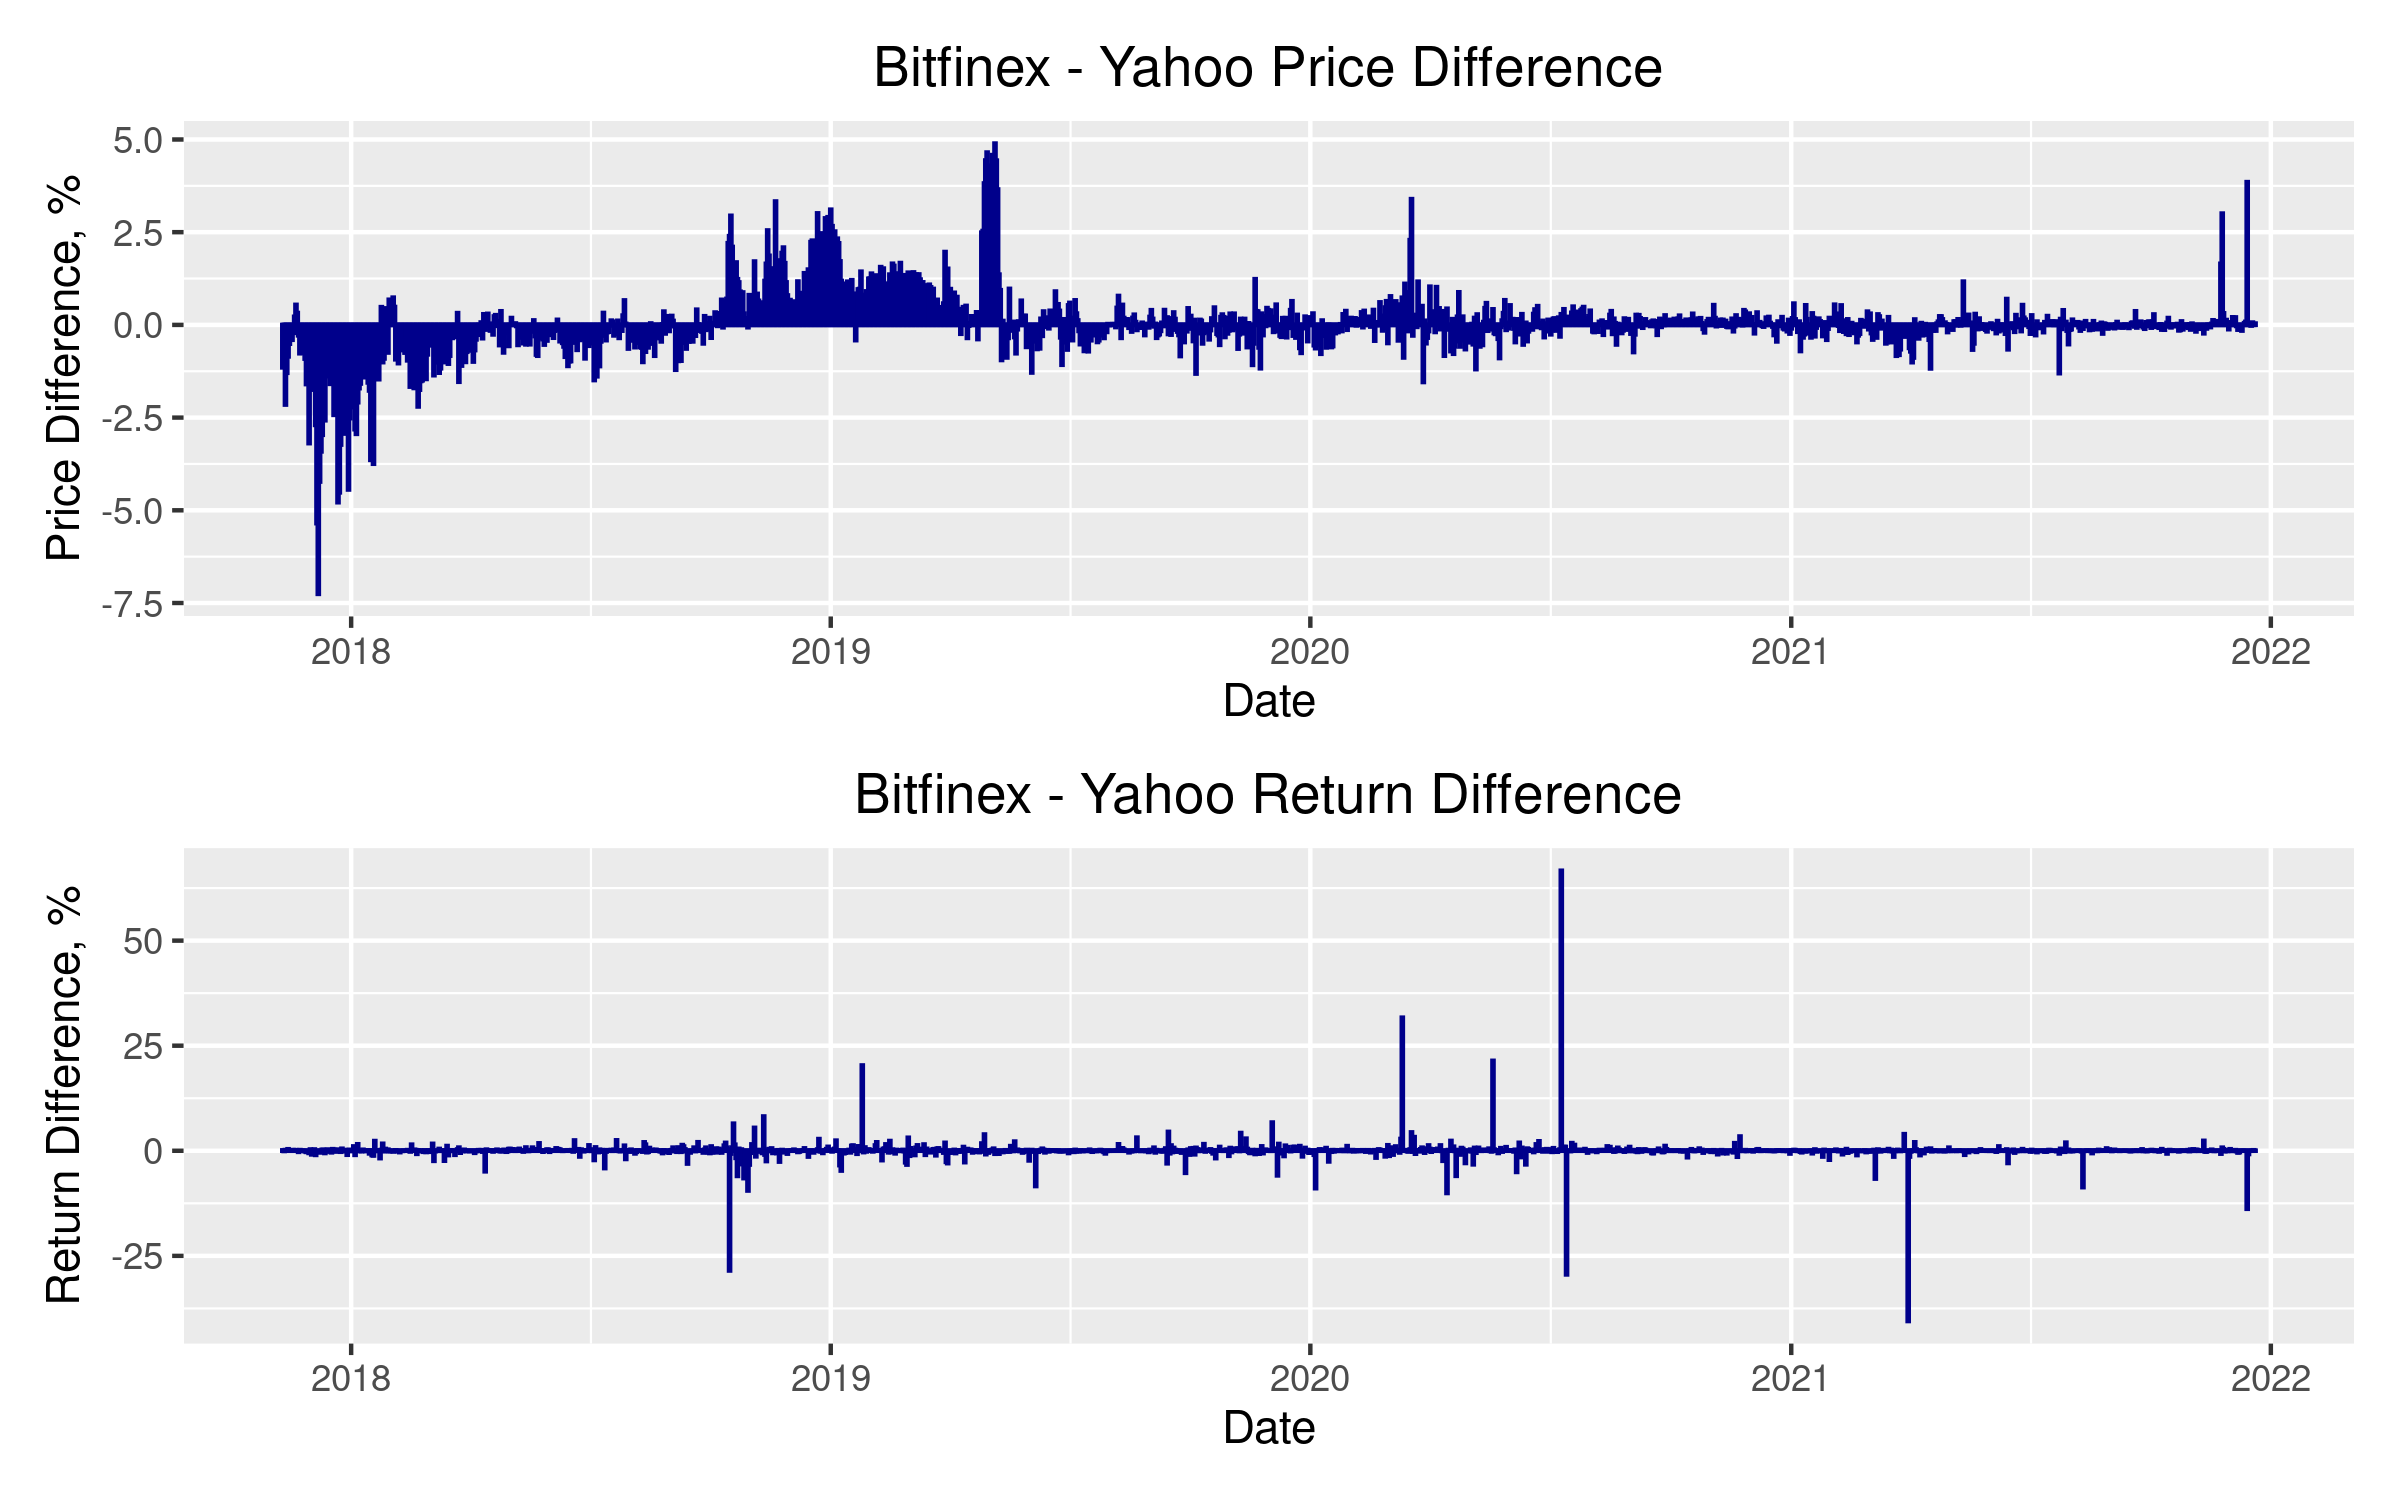
\includegraphics[scale=0.72]{{empirical_results/data_diff.png}}
	\subcaption*{Notes: Yahoo BTC-USD data is only available from November 10, 2018, while BitFinex BTC-USD data is available from January 01, 2015.}
\end{figure}

According to \cite{alexander2020critical}, more than 60$\%$ papers published in academic journals use data from unreliable sources, so-called price-tracking website. There are a lot of inconsistencies among traded prices on different sources. We sourced BTC-USD data from 2 popular sources: BitFinex and Yahoo Finance. Figure \ref{figure:price_diff} shows the differences in percentage of daily reported closing prices, and derived log-return between 2 sources. Interestingly, price differences are not random, especially for the period of 2018 to mid-2019, indicating some systematic differences in either data collection, consolidation, or reporting. Differences in returns can sometimes be very substantial: in some cases reach $\pm$25$\%$. In the end, we go with data from BitFinex due to higher availability. Data used is daily closing prices of Bitcoin (in \$) from 2015-01-01 to 2021-12-20, for a total of 2,543 observations.

% Please add the following required packages to your document preamble:
% \usepackage{booktabs}
\begin{table}[!htbp]
\begin{threeparttable}
\caption{Summary statistics of Bitcoin percentage log-returns}
\label{table:summarystats}
\begin{tabular}{@{}ccccccccc@{}}
\toprule
\textbf{Min} & \textbf{Max} & \textbf{Mean} & \textbf{Median} & \textbf{Std}  & \textbf{Skewness} & \textbf{Kurtosis} & \textbf{Jb $p$-val} \\ \midrule
-48.09     & 23.72       & 0.197     & 0.176       & 4.078          & -0.966        & 12.792            & 0                 \\ \bottomrule
\end{tabular}
\begin{tablenotes}
\small
\item Notes: The total number of returns is 2,543. Max stands for maximum; Min for minimum; Std for Standard deviation; Skew for Skewness; Kurt for Kurtosis and Jb for Jarque-Bera Normality test.
\end{tablenotes}
\end{threeparttable}
\end{table}

Table \ref{table:summarystats} describes some descriptive statistics of Bitcoin returns. In particular, kurtosis is $12.8$ and skewness is $-0.966$, which show that returns are leptokurtic and negative skewed. Together with the value of JB $p$-value, being equal to 0, it shows that Bitcoin returns are not normally distributed. As we can see from Figure \ref{figure:acf}, there is no strong evidence that indicates autocorrelation. However, the ACF of the absolute returns shows long diminishing autocorrelation over many lags, indicating possible variance clustering, where large changes happen close to each other. Furthermore, figure percentage log-returns of Figure \ref{figure:hist_price} confirms conditional heteroscedasticity. The annualized empirical volatility is $\sqrt{365} \times 4.08 = 78\%$.\par

\begin{figure}[h]
	\caption{Summary statistics of Bitcoin percentage log-returns}
	\label{figure:hist_price}
	\centering
	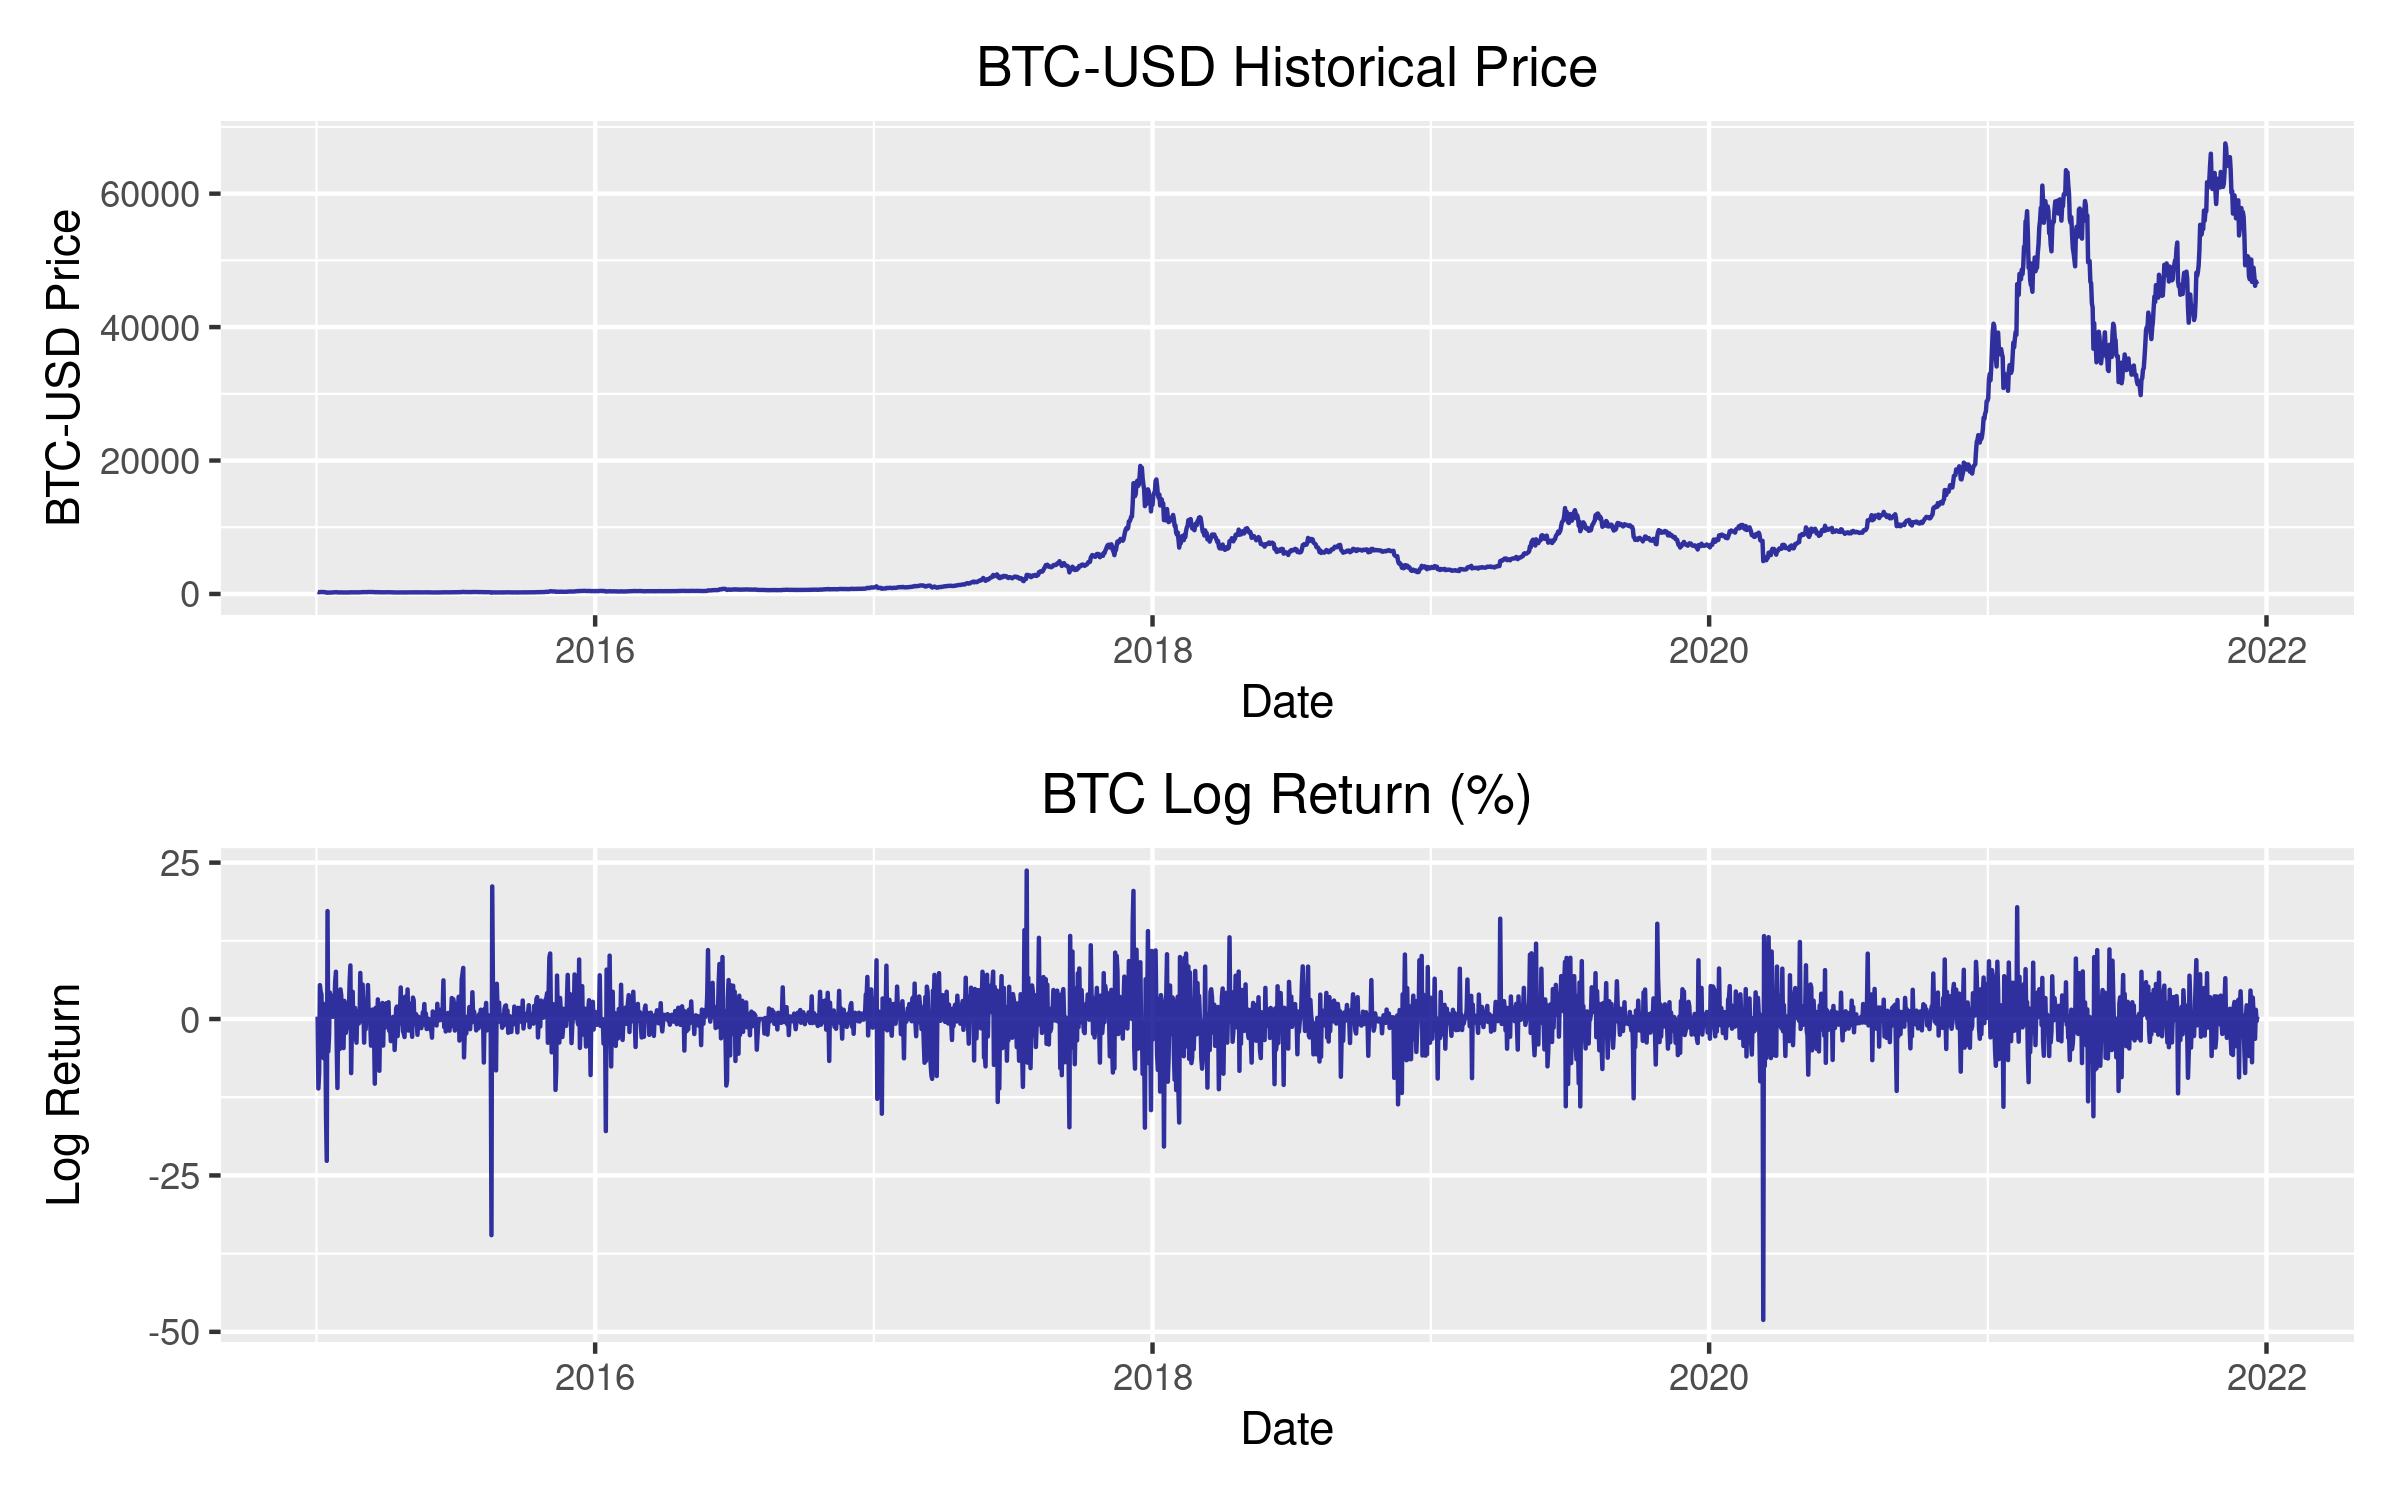
\includegraphics[scale=0.72]{{empirical_results/price_return.png}}
	\subcaption*{Notes: The time series range from January 01, 2015 to Dec 20, 2021 for the closing prices shown in the upper plot and from January 01, 2015 to Dec 20, 2021 for the percentage log-returns in the lower plot}
\end{figure}

\subsection{In-sample Analysis}
We will first begin with the in-sample analysis, in which 18 models are fitted to the whole dataset of demeaned and AR(1)-filtered log returns using  Maximum Likelihood Estimation (MLE). To assess the model's goodness-of-fit for models estimated with MLE, Akaike Information Criterion (AIC) \citep{akaike1998information} and Bayesian Information Criterion (BIC) \citep{schwarz1978estimating} will be used to select the most appropriate model in terms of a trade-off between the goodness of fit and the number of parameters \citep{guidolin2018essentials}. In addition to MLE, Bayesian Estimation can also be used to estimate parameters of MSGARCH models, and can bring good results \citep{ardia2019regime}. In order to verify this, the same routines and tests will also be done with the aforementioned models, estimated using Bayesian Estimation (BE). Since the posterior distribution of parameters do not have an analytical form, we sample estimated parameters using Markov Chain Monte Carlo (MCMC) methods \citep{ardia2019msgarchr}. On this front, Deviance Information Criterion (DIC) is used to evaluate goodness-of-fit \citep{spiegelhalter2002bayesian}.

As we can see from Table \ref{table:aicbic}, for all distribution and variance specifications, except for the case GJR(2)-sk$\mathcal{S}$ model, MSG(K) models in both 2 and 3 regimes almost outperform SRG models, which is the same as the conclusions of \cite{ardia2019regime} and \cite{maciel2021cryptocurrencies}. Particularly, for all states, sGARCH models display lower values than GJR-GARCH. Regarding the volatility specifications, the best in-sample models are sGARCH(2)-sk$\mathcal{S}$ model and sGARCH(3)-sk$\mathcal{S}$ model based on AIC, which shows no evidence of inverted leverage effects. Bayesian Estimation, on the other hand, prefers GJR-GARCH with three regimes.\par


\begin{landscape}
\begin{table}[]
\center
\begin{threeparttable}
\caption{In-sample model selection for Bitcoin}
\label{table:aicbic}
\begin{tabular}{lccclccclccc}
\hline
          & \multicolumn{3}{c}{$\mathcal{N}$} & \multicolumn{1}{c}{} & \multicolumn{3}{c}{$\mathcal{S}$}    &                      & \multicolumn{3}{c}{sk$\mathcal{S}$}          \\
Model     & AIC       & BIC       & DIC       & \multicolumn{1}{c}{} & AIC     & BIC              & DIC     & \multicolumn{1}{c}{} & AIC              & BIC     & DIC              \\ \hline
\multicolumn{12}{c}{\textit{Regime $k=1$}}                                                                                                                                         \\
sGARCH    & 14004.3   & 14021.9   & 14004.8   &                      & 13245.0 & 13268.4          & 13246.0 &                      & 13240.5          & 13269.7 & 13241.4          \\
GJR-GARCH & 13988.5   & 14011.9   & 13988.4   &                      & 13247.0 & 13276.3          & 13250.4 &                      & 13242.6          & 13277.6 & 13276.5          \\
\multicolumn{12}{c}{\textit{Regime $k=2$}}                                                                                                                                         \\
sGARCH    & 13302.1   & 13348.9   & 13304.1   &                      & 13170.7 & 13220.7          & 13220.7 &                      & \textbf{13164.1} & 13234.2 & 13205.2          \\
GJR-GARCH & 13455.5   & 13513.9   & 13304.1   &                      & 13199.8 & \textbf{13209.9} & 13209.9 &                      & 13329.6          & 13411.3 & 13199.0          \\
\multicolumn{12}{c}{\textit{Regime $k=3$}}                                                                                                                                         \\
sGARCH    & 13236.8   & 13324.4   & 13339.6   &                      & 13174.8 & 13279.9          & 13215.1 &                      & 13168.6 & 13291.3 & 13297.0          \\
GJR-GARCH & 13352.6   & 13457.7   & 13277.6   &                      & 13189.5 & 13312.1          & 38241.3 &                      & 13174.8          & 13315.0 & \textbf{13183.5} \\ \hline
\end{tabular}
\begin{tablenotes}
\small
\item Notes: The table reports the Bayesian information criterion (BIC) and the Akaike information criterion (AIC) for the 18 specified models. The smallest values are printed in bold and highlight the best in-sample models. sGARCH is the symmetric GARCH of Bollerslev (1986) and GJR is the asymmetric GARCH model of Glosten et al. (1993). $\mathcal{N}$ , $\mathcal{S}$ and sk$\mathcal{S}$ are the standard normal, standardized Student's t-distribution and standardized skewed-Student's t-distribution, respectively.
\end{tablenotes}
\end{threeparttable}
\end{table}
\end{landscape}

According to the result from Table \ref{table:aicbic}, the parameter estimates of the best in-sample model, namely sGARCH(2)-sk$\mathcal{S}$, and its counterpart are presented in Table \ref{table:params_ml}. $\omega_k$, $\alpha_k$, $\beta_k$ are the sGARCH parameters, $\nu_k$ is the tail parameters and $\delta_k$ is the asymmetry parameter of the standardized skewed Student's t-distribution in regime $k$. $\nu_1$ and $\delta_1$ indicate excess kurtosis and right skewness, respectively. The sum of $\alpha_1$ and $\beta_1$ is close to 1, indicating high persistence of the volatility dynamics.

\begin{table}[tb]
\small
\center
\begin{threeparttable}
\caption{Parameter estimates}
\label{table:params_ml}
\begin{tabular}{lllllll}
\hline
               & \multicolumn{2}{c}{Single-regime} & \multicolumn{2}{c}{Two-regime} & \multicolumn{2}{c}{Three-regime} \\ \hline
\multicolumn{6}{l}{\textit{Regime $k=1$}}                                                        &                     \\
$\omega_1$     & 0.1967***        & (0.0627)       & 0.9424***      & (0.3635)      & 0***       & $(<1\mathrm{e}-10)$ \\
$\alpha_1$     & 0.1115*          & (0.0731)       & 0.0721**       & (0.0413)      & 0.0145***  & $(<1\mathrm{e}-10)$ \\
$\beta_1$      & 0.8873***        & (0.0008)       & 0.8924***      & (0.0178)      & 0.9854***  & $(<1\mathrm{e}-10)$ \\
$\nu_1$        & 3.3585***        & (0.1494)       & 5.2787***      & (1.0495)      & 2.8459***  & $(<1\mathrm{e}-10)$ \\
$\delta_1$     & 0.9513***        & (0.0187)       & 0.9149***      & (0.0324)      & 0.9344***  & $(<1\mathrm{e}-10)$ \\
$p_11$         & 1                &                & 0.9877         &               & 0.9762     &                     \\
$\text{aUV}_1$ & 89.2114          &                & 98.1903        &               & 0.6639     &                     \\ \hline
\multicolumn{6}{l}{\textit{Regime $k=2$}}                                                        &                     \\
$\omega_2$     & -                &                & 0.2971**       & (0.1467)      & 0.0038***  & $(<1\mathrm{e}-10)$ \\
$\alpha_2$     & -                &                & 0.0781         & (0.061)       & 0.0098***  & $(<1\mathrm{e}-10)$ \\
$\beta_2$      & -                &                & 0.9213***      & (0.0004)      & 0.9842***  & $(<1\mathrm{e}-10)$ \\
$\nu_2$        & -                &                & 2.3258***      & (0.0814)      & 2.2125***  & $(<1\mathrm{e}-10)$ \\
$\delta_2$     & -                &                & 0.954***       & (0.027)       & 1.0019***  & $(<1\mathrm{e}-10)$ \\
$p_22$         & -                &                & 0.9848         &               & 0.9720     &                     \\
$text{aUV}_2$  & -                &                & 59.2302        &               & 9.4739     &                     \\ \hline
\multicolumn{6}{l}{\textit{Regime $k=3$}}                                                        &                     \\
$\omega_3$     & -                &                & -              &               & 4.0207***  & $(<1\mathrm{e}-10)$ \\
$\alpha_3$     & -                &                & -              &               & 0.0958***  & $(<1\mathrm{e}-10)$ \\
$\beta_3$      & -                &                & -              &               & 0.7831***  & $(<1\mathrm{e}-10)$ \\
$\nu_3$        & -                &                & -              &               & 5.6673***  & $(<1\mathrm{e}-10)$ \\
$\delta_3$     & -                &                & -              &               & 0.8618***  & $(<1\mathrm{e}-10)$ \\
$p_33$         & -                &                & -              &               & 0.9803     &                     \\
$\text{aUV}_3$ & -                &                & -              &               & 110.1367   &                     \\ \hline
\end{tabular}
\begin{tablenotes}
\small
\item Notes: The table presents the maximum-likelihood parameter estimates of the $K$-regime sGARCH-skS models, K = 1; 2; 3. sGARCH is the symmetric GARCH model of Bollerslev (1986). skS is the standardized skewed Student's t-distribution with tail parameter $\nu$ and asymmetry parameter $\delta$. $p_{kk}$ is the staying probability of state $k$. $aUV$ is the annualized unconditional volatility (in $\%$). In parentheses are the standard errors. *, **, and *** indicate significance at the 10$\%$, 5$\%$ and 1$\%$ levels, respectively
\end{tablenotes}
\end{threeparttable}
\end{table}

Unlike \cite{ardia2019regime}, we find that a MSG(2) and skewed Student's t-distribution to be the best in-sample model based on AIC. While BIC points to standard Student's t-distribution, two-regime is still the common ground, indicating that volatility process can switch between two regimes. And since standard Student's t-distribution is a special case of skewed Student's t-distribution, we can make use of the latter. The MSG(2) parameters show that the BTC volatility process switch between a low- and high-volatility regime with an annualized uncondition volatility. of 99$\%$ in regime 1 and 54$\%$ in regime 2. Both regimes are extremely durable with the staying probabilities $p_{kk} = 0.98$, $k = 1,2$. On average, low- and high-volatility regimes are equally likely as indicated by the stable probabilities $\lambda_1 = 0.55$ and $\lambda_2 = 0.45$. In particular, $\omega_2$ is considerably smaller than $\omega_1$, which shows the same pattern as annualized unconditional volatility between two states. Further, both $\alpha_2$ and $\beta_2$ are higher than $\alpha_1$ and $\beta_1$, indicating a stronger reaction to shocks and more volatility memory in the low-volatility regime. This situation can be presumably explained by finding of \cite{haas2004new}, the effect of the pressured market circumstances, COVID-19 to the market. The estimated probability transition matrix of the sGARCH(2)-sk$\mathcal{S}$ model is:
\begin{align}
P = \begin{bmatrix} 0.9877 & 0.0123 \\ 0.0152 & 0.9848 \end{bmatrix}
\end{align}

To understand more about the volatility regimes of BTC-USD returns, we can use the estimated probability of being in a certain regime for certain points in time \citep{guidolin2018essentials}, here denoted $z_{k,t\vert \Psi , \mathcal{I}}$. There are 2 types of probabilities indicating current regimes: filtered probability and smoothed probability. Filtered probability $z_{k,t\vert \Psi , \mathcal{I}_{t-1}}$, which is a real-time inference on the state probabilities, depends only on information up to time $t$. Smoothed probability $z_{k,t\vert \Psi , \mathcal{I}_{T}}$, on the other hand, depends on the entire information set available, and is more suitable for retrospective analysis conducted here. Figure \ref{figure:smooth_probs_ml} shows the ML-estimated smoothed probability of returns being in high-volatility regime $k = 1$. There are 2 long periods that has continuously high (smoothed) probability of being in the high-volatility regime, that is around the year 2017 to 2019, and from 2021 to 2022. This aligns quite well with the development ob BTC-USD price, which exhibited wild fluctuation during the same periods.

\begin{figure}[h]
	\caption{Smoothed probabilities and annualized volatilities}
	\label{figure:smooth_probs_ml}
	\centering
	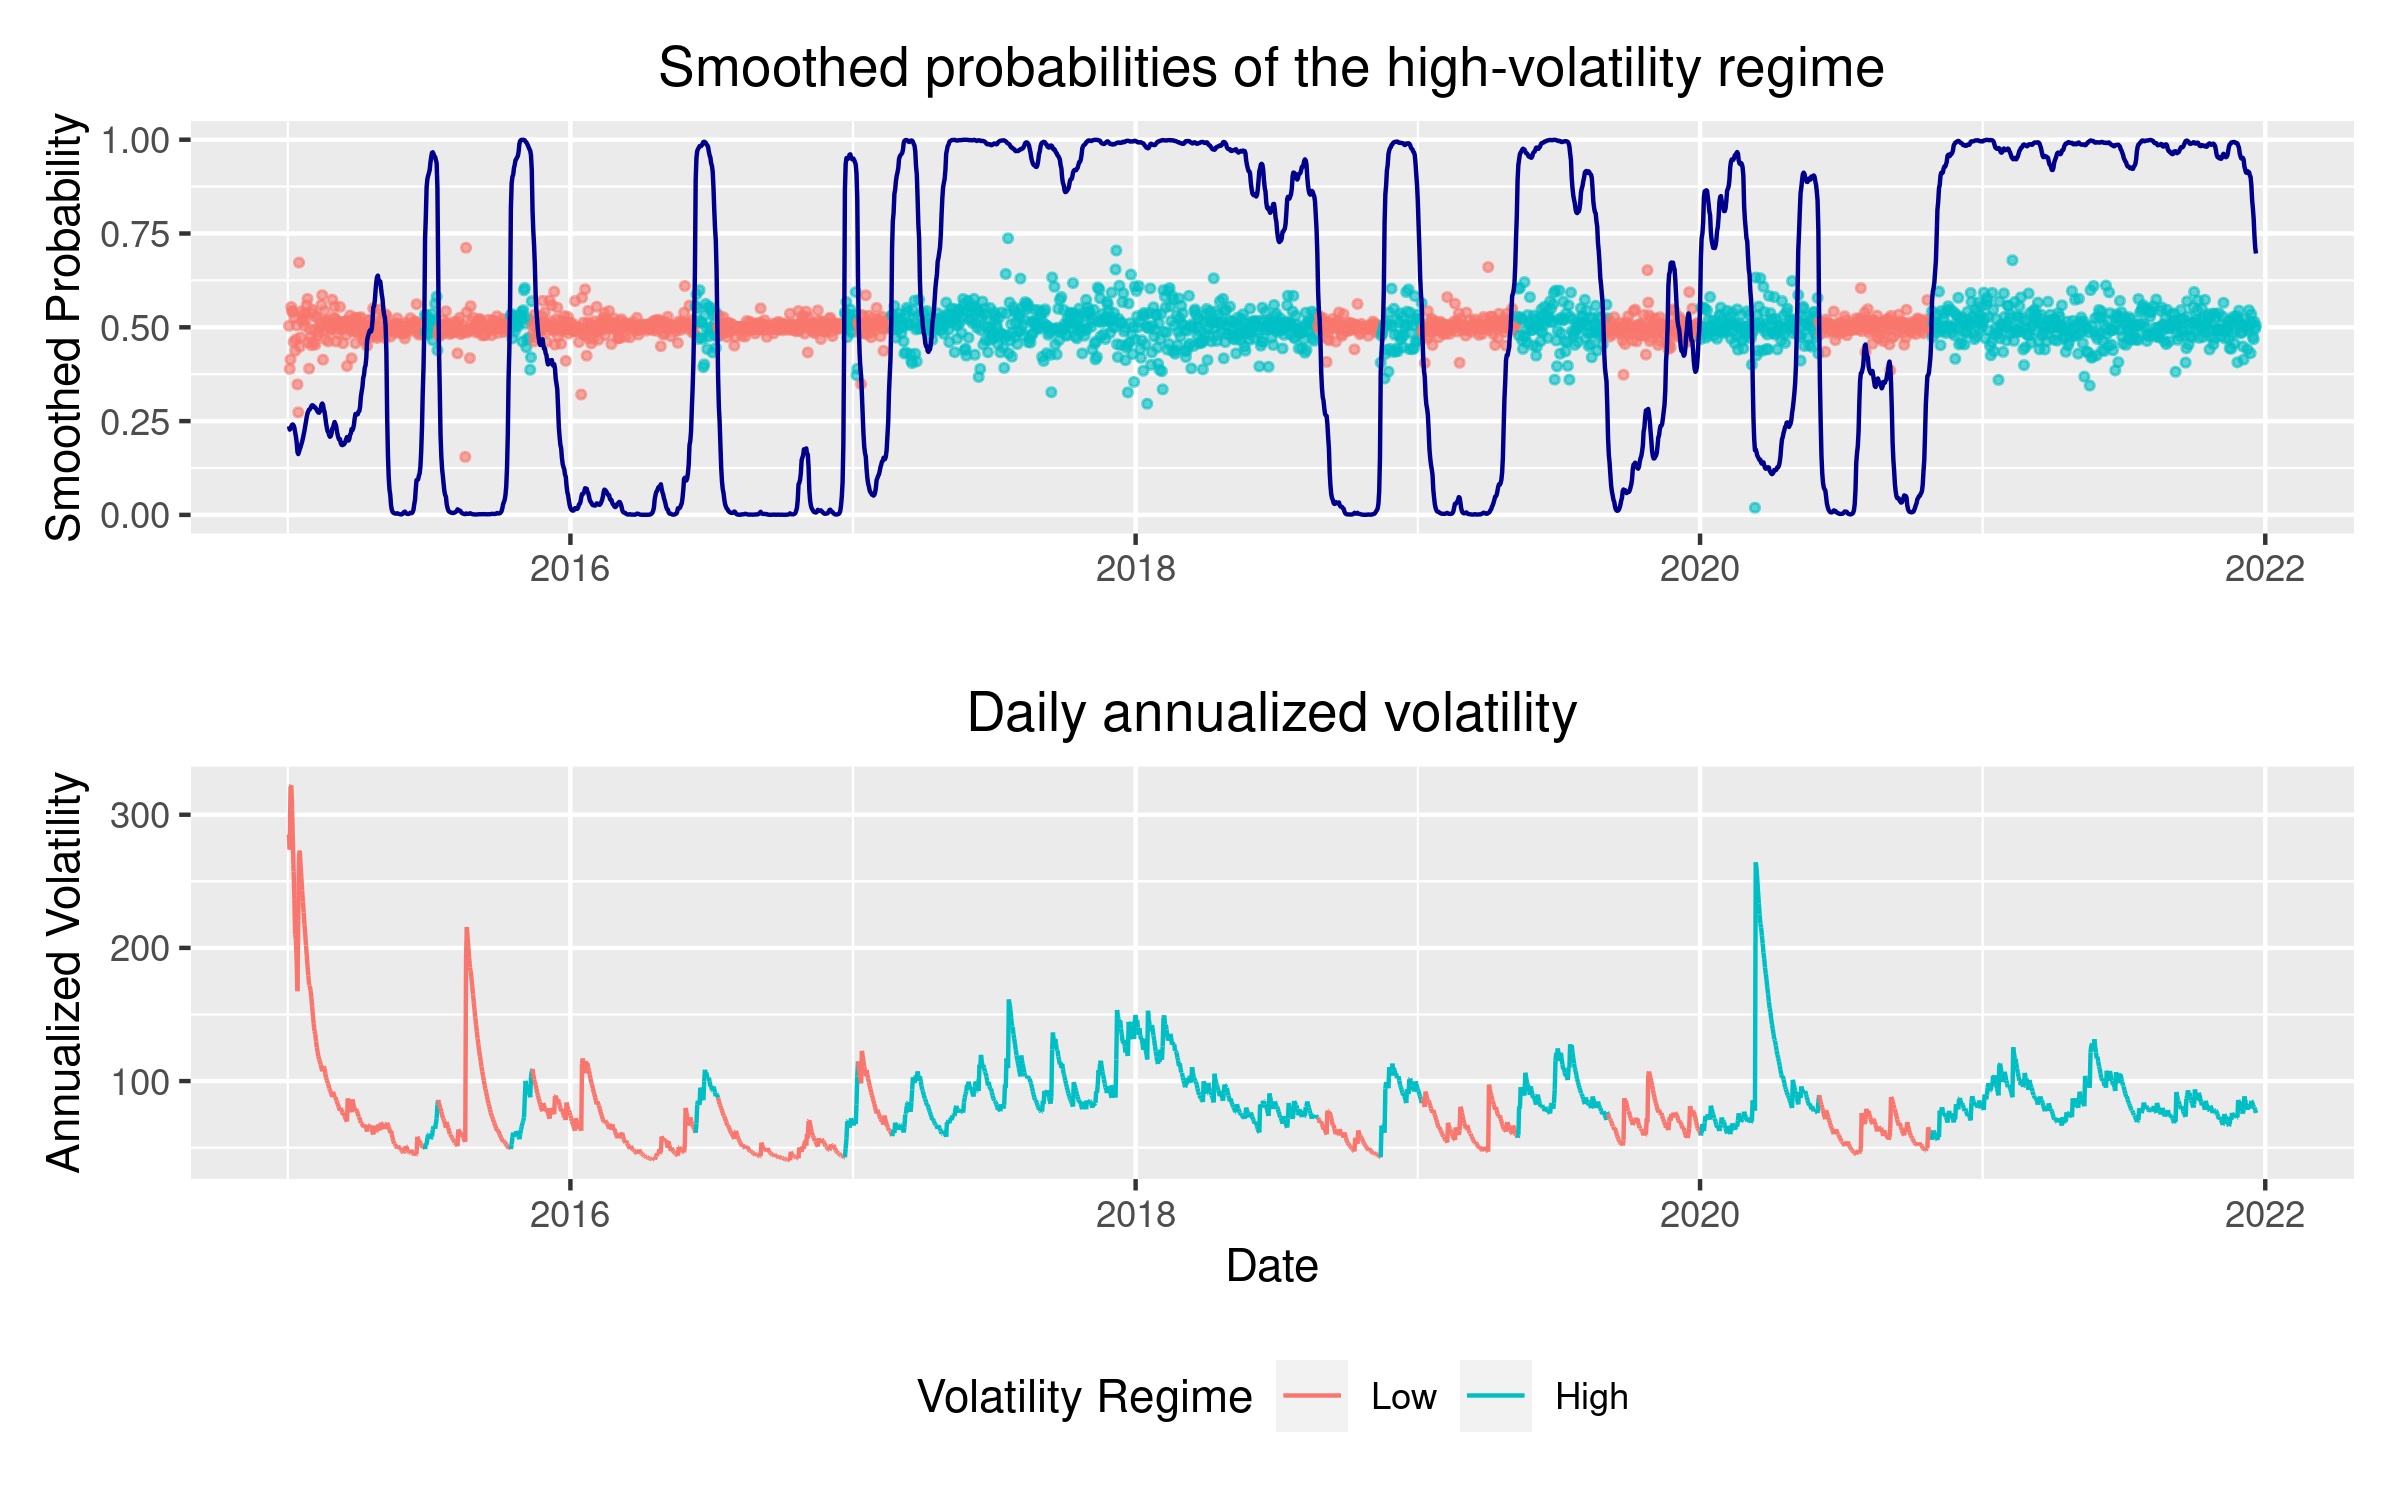
\includegraphics[scale=0.73]{{empirical_results/prob_vol_plot.png}}
	\subcaption*{Notes: The time series range from January 01, 2015 to Dec 20, 2021. The graphs are computed from the two-regime sGARCH model with a standardized skewed Student's t-distribution. Parameters in the models are estimated using MLE. The estimated smoothed probabilities of the high-volatility regime (1st regime) are shown in the upper graph and the BTC log-returns (points). The bottom graph shows the annualized volatilities in percentage. The colors of each point and color segments of the annualized volatility series indicate the regime to which the points or segments are predicted to belong.}
\end{figure}

As for Bayesian Estimation, our largest model in the repertoire achieves the lower DIC, hence is used for in-sample analysis. The chosen model has GJR-GARCH as the underlying process for return volatility, which has a leverage effect parameter $\gamma$, and is inline with findings from \cite{ardia2019regime}. $K = 3$ indicates that the volatility process of out BTC-USD returns follows 3 distinct regimes, which low ($26.98\%$), medium ($71.18\%$), and high ($123.7\%$) unconditional volatility, as shown in Table \ref{table:params_mcmc}. In-sample predicted smoothed probability shows that this model specification changes regimes very eagerly and disruptively, without staying at one regime for too long. As can be seen in Figure \ref{figure:smooth_probs_mcmc}, the model stays medium-volatility regime the most, followed by relatively long periods of low-volatility regime. High-volatility regime, on the other hand, appears sparsely and only shortly, interloping between medium-volatility periods.

\subsection{Out-of-sample Analysis}
For out-of-sample analysis, we use a rolling window of size 2,189 for both MLE and BE. We construct 354 out-of-sample one-step VaR predictions from January 01, 2021 to December 20, 2021. We update the parameters of our models after every five one-step-ahead forecasts. The reason we use a rather large rolling window for estimation is to see if data in the long past can be indicative of recent record-breaking swings in BTC-USD returns. In 2021 alone, BTC-USD prices went from around \$30,000 to more than \$60,000, then crashed back to \$30,000 before spiking up to yet another new record of around \$68,000 and slid down from there.

\begin{figure}[!htb]
    \caption{Value-at-risk forecasts}
    \label{figure:oos_var_ml}
    \centering
    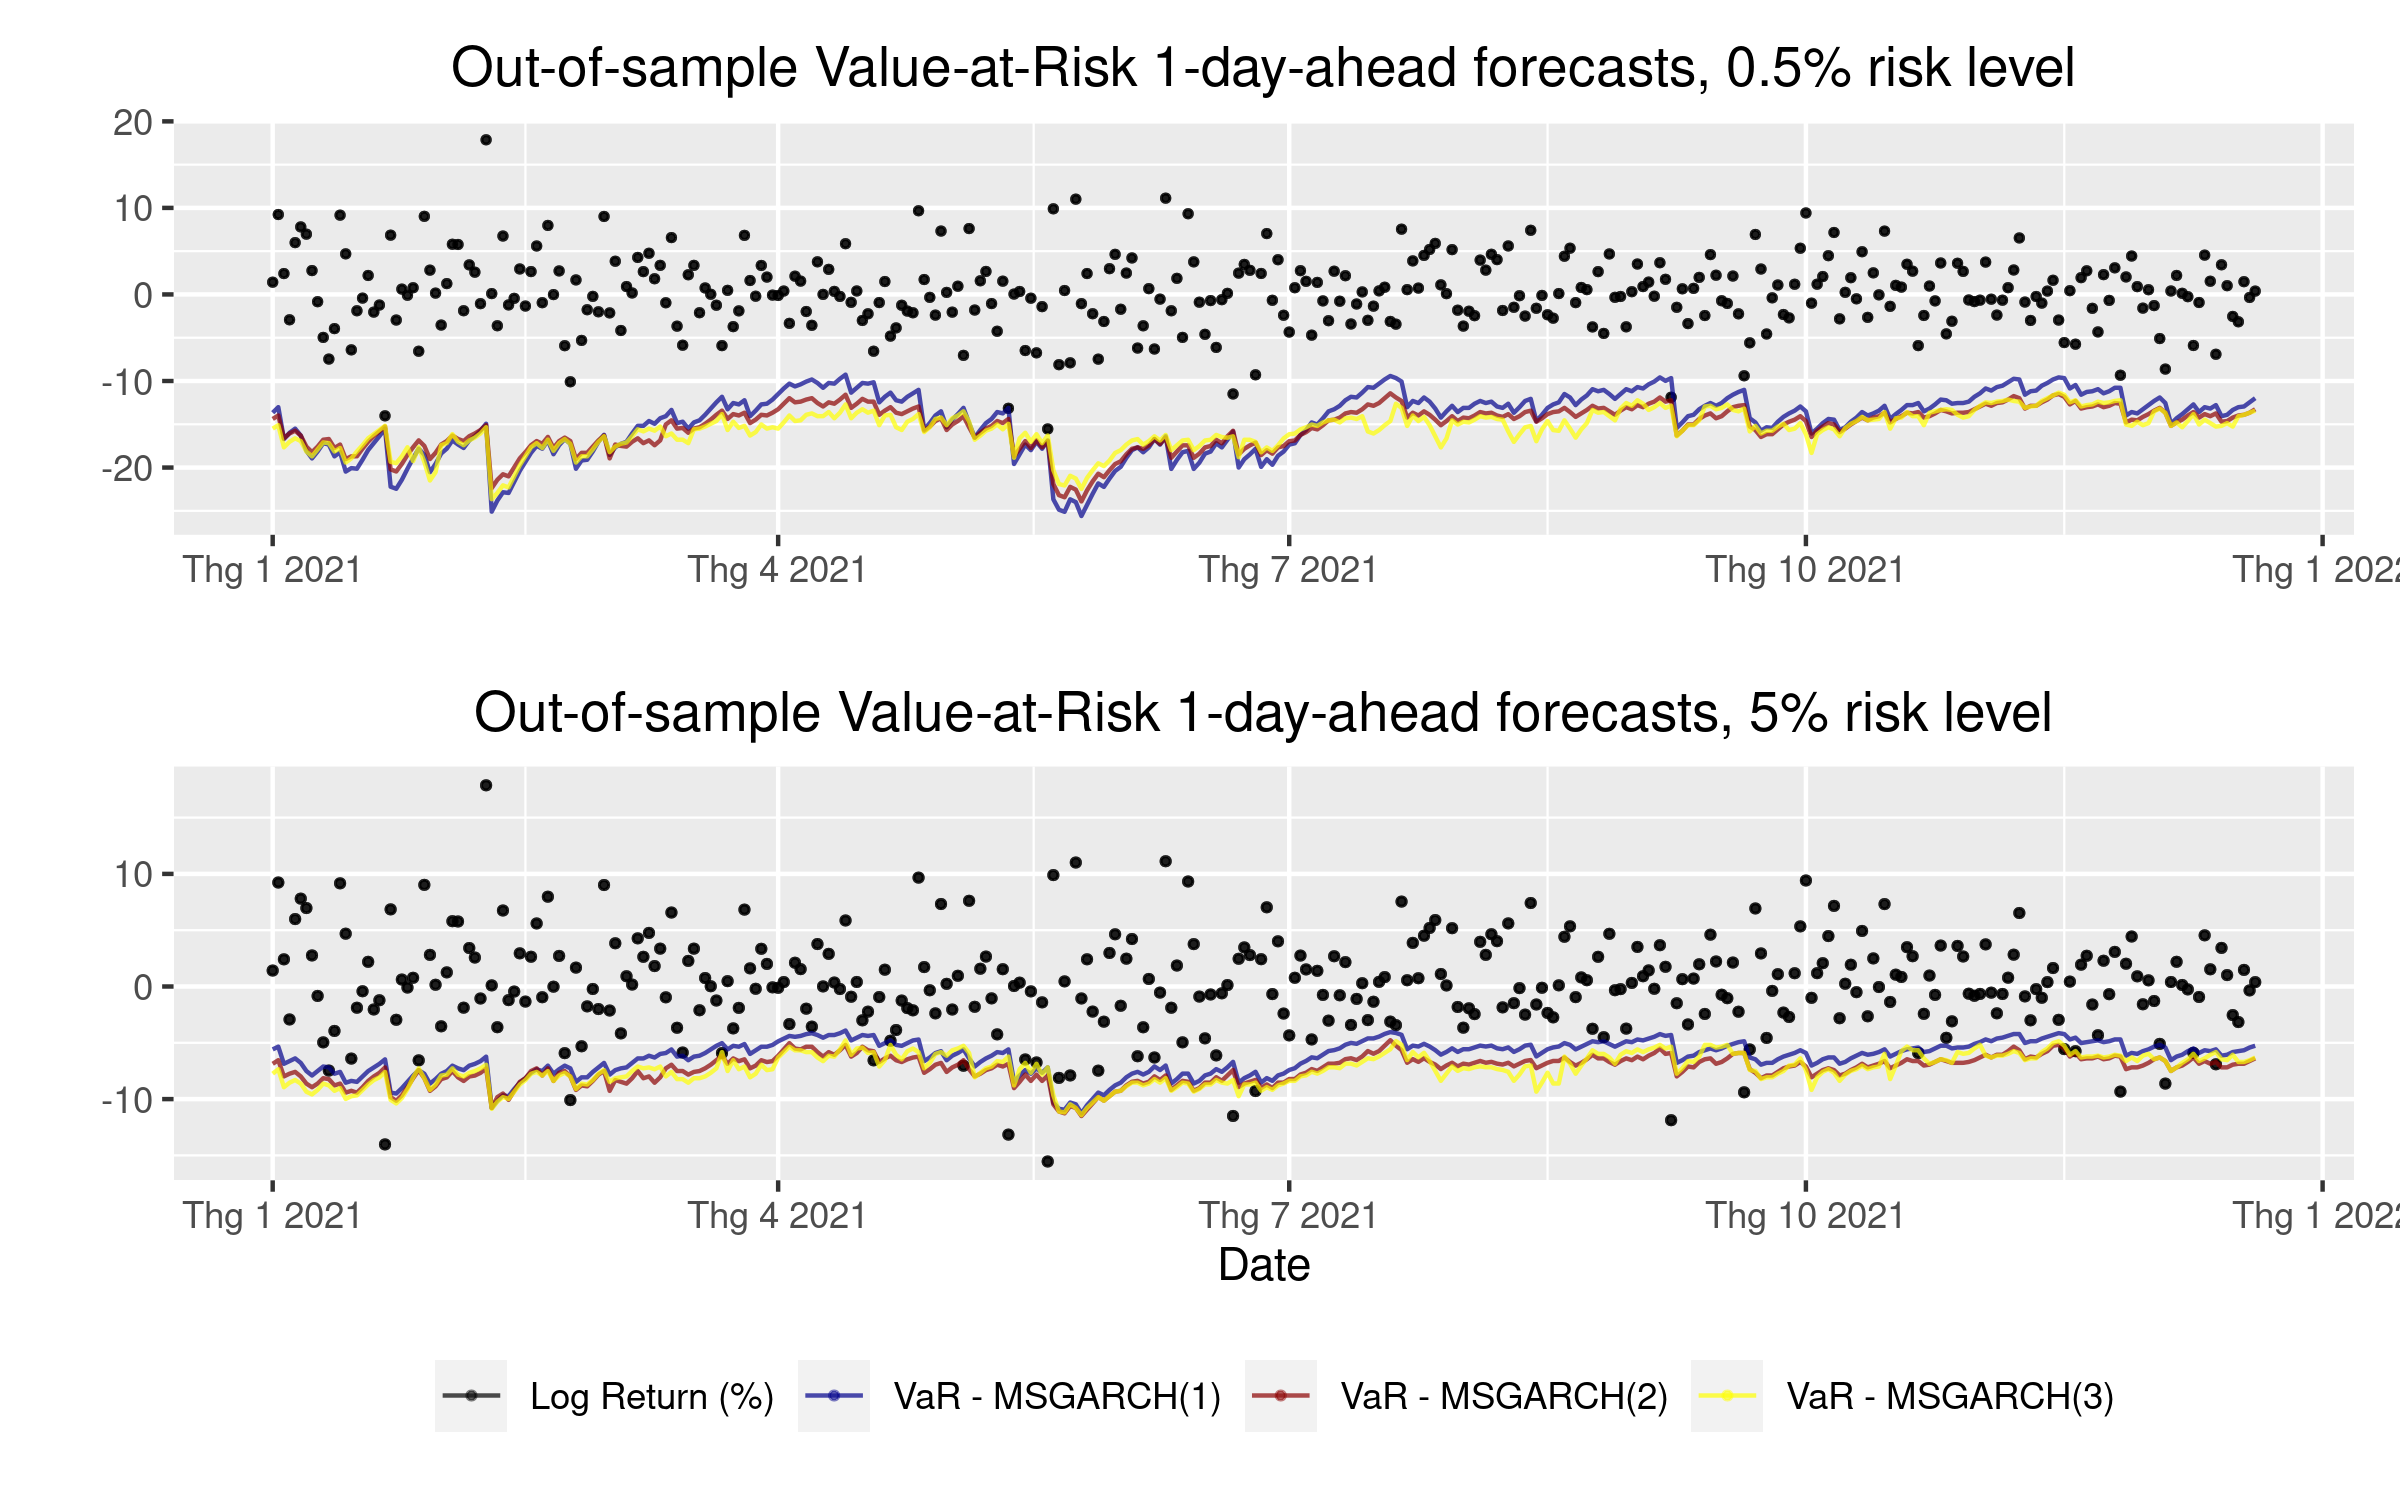
\includegraphics[scale=0.73]{{empirical_results/oos_VaR.png}}
    \subcaption* {Notes: The time series range from January 01, 2015 to Dec 20, 2021. The out-of-sample period ranges from Jan 01, 2021 to Dec 20, 2021. The top graph shows the one-day-ahead Value-at-risk (VaR) forecasts at the 0.5$\%$ risk level computed with the single regime (blue line), two-regime (red line) and three-regime (green line) sGARCH-sk$\mathcal{S}$ model. The percentage log-returns are depicted as the dots. sGARCH is the symmetric GARCH model of \cite{bollerslev1986generalized} and sk$\mathcal{S}$ is the standardized skewed Student's t-distribution. The bottom graph depicts the one-day-ahead VaR forecasts at the 5$\%$ risk level. The single-regime GARCH tends to lead to (absolute) smaller VaR values and thus, the observed number of violations is higher than for the two-regime GARCH model.}
\end{figure}


Table \ref{table:backtest_ml} presents the backtesting results for one-step-ahead VaR at the 0.5$\%$, 1$\%$, 5$\%$ and 10$\%$ risk levels. As mentioned above, the purpose of backtesting here is to consider whether the VaR calculation in practice is significantly dfferent from VaR from model estimation. We can see that among three regimes, single-regime GARCH have more rejections than two- and three-regime GARCH. Both $LR_{UC}$ and $LR_{CC}$ test reject the adequacy of MSGARCH(1) at the 5$\%$ and 10$\%$ level of significance for the 10$\%$ risk level.  Moreover, we also reject the null hypothesis of correct VaR forecasting for two–regime and three–regime MSGARCH models for the 0.5$\%$ VaR at the 10$\%$ level of significance. According to findings of \cite{ardia2019regime}, \cite{maciel2021cryptocurrencies}, SGR model is not a valid risk model since it underestimates the BTC risk. However, based on the result in Table \ref{table:hitrate}, it seems that all three models have almost the same power in detecting the VaR violations. Particularly, in Table \ref{table:hitrate}, the number of hits  of three models are all lower than the expected number of hits for all risk levels. Again, this can be seen graphically in Figure \ref{figure:oos_var_ml}. We can conclude that the models tend to overestimate the BTC risk, which contradicts to the findings of \cite{ardia2019regime}. \par

\begin{table}[]
\centering
\begin{threeparttable}
\caption {Backtesting results for 1-step-ahead volatility forecasts}
\label{table:backtest_ml}
\begin{tabular}{@{}lllclclclcl@{}}
\toprule
           & \multicolumn{2}{l}{VaR risk level} & \multicolumn{2}{c}{0.005}           & \multicolumn{2}{c}{0.01}   & \multicolumn{2}{c}{0.05}   & \multicolumn{2}{c}{0.1}             \\ \midrule
MSGARCH(1) & \multicolumn{2}{c}{$LR_{UC}$}      & \multicolumn{2}{c}{0.8652}          & \multicolumn{2}{c}{0.2319} & \multicolumn{2}{c}{0.5823} & \multicolumn{2}{c}{\textbf{0.0220}} \\
           & \multicolumn{2}{c}{$LR_{CC}$}      & \multicolumn{2}{c}{0.9745}          & \multicolumn{2}{c}{0.4412} & \multicolumn{2}{c}{0.2584} & \multicolumn{2}{c}{\textbf{0.0722}} \\
MSGARCH(2) & \multicolumn{2}{c}{$LR_{UC}$}      & \multicolumn{2}{c}{\textbf{0.0596}} & \multicolumn{2}{c}{0.8098} & \multicolumn{2}{c}{0.3498} & \multicolumn{2}{c}{0.6675}          \\
           & \multicolumn{2}{c}{$LR_{CC}$}      & \multicolumn{2}{c}{0.1696}          & \multicolumn{2}{c}{0.9279} & \multicolumn{2}{c}{0.3622} & \multicolumn{2}{c}{0.9105}          \\
MSGARCH(3) & \multicolumn{2}{c}{$LR_{UC}$}      & \multicolumn{2}{c}{\textbf{0.0596}} & \multicolumn{2}{c}{0.8098} & \multicolumn{2}{c}{0.8636} & \multicolumn{2}{c}{0.6675}          \\
           & \multicolumn{2}{c}{$LR_{CC}$}      & \multicolumn{2}{c}{0.1696}          & \multicolumn{2}{c}{0.9279} & \multicolumn{2}{c}{0.4168} & \multicolumn{2}{c}{0.9105}          \\ \bottomrule
\end{tabular}
\begin{tablenotes}
\small
\item Notes: The table presents the backtesting results for the 1-step-ahead value-at-risk ( VaR ) at risk levels 0.5$\%$, 1$\%$, 5$\%$ and 10$\%$. Shown are the p-values of the Likelihood Ratio test of Unconditional Coverage $(LR_{UC})$ and the Likelihood Ratio test of Conditional Coverage $(LR_{CC})$ for the K-regime symmetric sGARCH \citep{bollerslev1986generalized} models, K = 1,2,3, with a standardized skewed Student's t-distribution.
\end{tablenotes}
\end{threeparttable}
\end{table}

The models of which parameters are estimated with Bayesian method tell a similar story. According to Table \ref{table:backtest_mcmc}, the two- and three-regime models, however, see rejection of unconditional test, at 10$\%$ and 0.5$\%$ risk levels while single-regime model rejects both tests at 10$\%$ risk level. These test results stem from overestimation of risks for all models, more so for the multiple regime ones, showed in the Table \ref{table:hitrate}. Again, empirical results of \cite{ardia2019regime} disagree with the results here.

There are a few possible explanation for the disparity in empirical results. First, BTC-USD historical price data is obtained from different sources. As we have discussed earlier in this paper, the return differences derived from prices between sources can be substantial. Figure \ref{figure:price_diff} is a demonstration. secondly, the data periods used are different. Since 2018, BTC has experienced some significant growth in both popularity and value. In 2018, BTC-USD price peaked around less then \$20,000 and eventually hovers around \$7,000. BTC-USD reached \$60,000 in April 2021 before crashing down to \$32,000 in May 2021 and bounced back to more than \$65,000 towards the end of 2021 before another dip to \$50,000. Such consistent large swings may empirically favor a single high-volatility regime instead of multiple regimes. Lastly, the rolling window size used in our study may not be optimal, since  it includes a large portion of data from a relatively distant past, the signals of which may overpower more recent patterns in return volatility.

\begin{table}[htp]
\centering
\caption{Expected and observed number of violations}
\label{table:hitrate}
\begin{tabular}{@{}rlclclclcl@{}}
\toprule
\multicolumn{2}{r}{VaR risk level}     & \multicolumn{2}{c}{0.005} & \multicolumn{2}{c}{0.01}  & \multicolumn{2}{c}{0.05} & \multicolumn{2}{c}{0.1}   \\ \midrule
\multicolumn{2}{r}{\textit{Expected number of hits}} & \multicolumn{2}{c}{5.31}  & \multicolumn{2}{c}{10.62} & \multicolumn{2}{c}{53.1} & \multicolumn{2}{c}{106.2} \\
\multicolumn{2}{r}{\textit{Observed number of hits}} & \multicolumn{8}{c}{}                                                                                         \\
\multicolumn{2}{r}{MSGARCH(1)}         & \multicolumn{2}{c}{2}     & \multicolumn{2}{c}{6}     & \multicolumn{2}{c}{20}   & \multicolumn{2}{c}{49}    \\
\multicolumn{2}{r}{MSGARCH(2)}         & \multicolumn{2}{c}{0}     & \multicolumn{2}{c}{4}     & \multicolumn{2}{c}{14}   & \multicolumn{2}{c}{33}    \\
\multicolumn{2}{r}{MSGARCH(3)}         & \multicolumn{2}{c}{0}     & \multicolumn{2}{c}{4}     & \multicolumn{2}{c}{17}   & \multicolumn{2}{c}{33}    \\ \bottomrule
\end{tabular}
\end{table}


\section{Conclusion}
Taking recent rising popularity of Crytocurrencies, in particular Bitcoin, into account, it is crucial to select the accurate models for estimating risk. The aim of this paper is to assess whether there are regime changes in the BTC volatility dynamics. In-sample analyses highly favor multiple regimes for models estimated by either Maximum Likelihood Estimation or Bayesian estimation. Only BE points towards model with leverage effect using GJR-GARCH as the underlying process of return volatility. The backtesting results, on the other hand, are less decisive on the matter of single vs multiple regimes. In the out-of-sample analysis, 2- and 3-regime models selected and estimated by both MLE and BE only give somewhat better backtesting results at $10\%$ risk level, while single-regime model is slightly better at $0.5\%$ risk level. In all cases, models tend to overestimate risks for the backtesting period used. Our findings contradict that of relevant papers, such as \cite{ardia2019regime}, \cite{caporale2019modelling}, \cite{maciel2021cryptocurrencies}. The differences may be attributed to different amount of data used, different backtesting period, and rolling window size used for parameter estimation.


\newpage
\bibliographystyle{chicago}
\bibliography{thesis_citation}


\newpage
\section{Appendix}

\begin{figure}[!htbp]
	\caption{Autocorrelation Functions}
	\label{figure:acf}
	\centering
	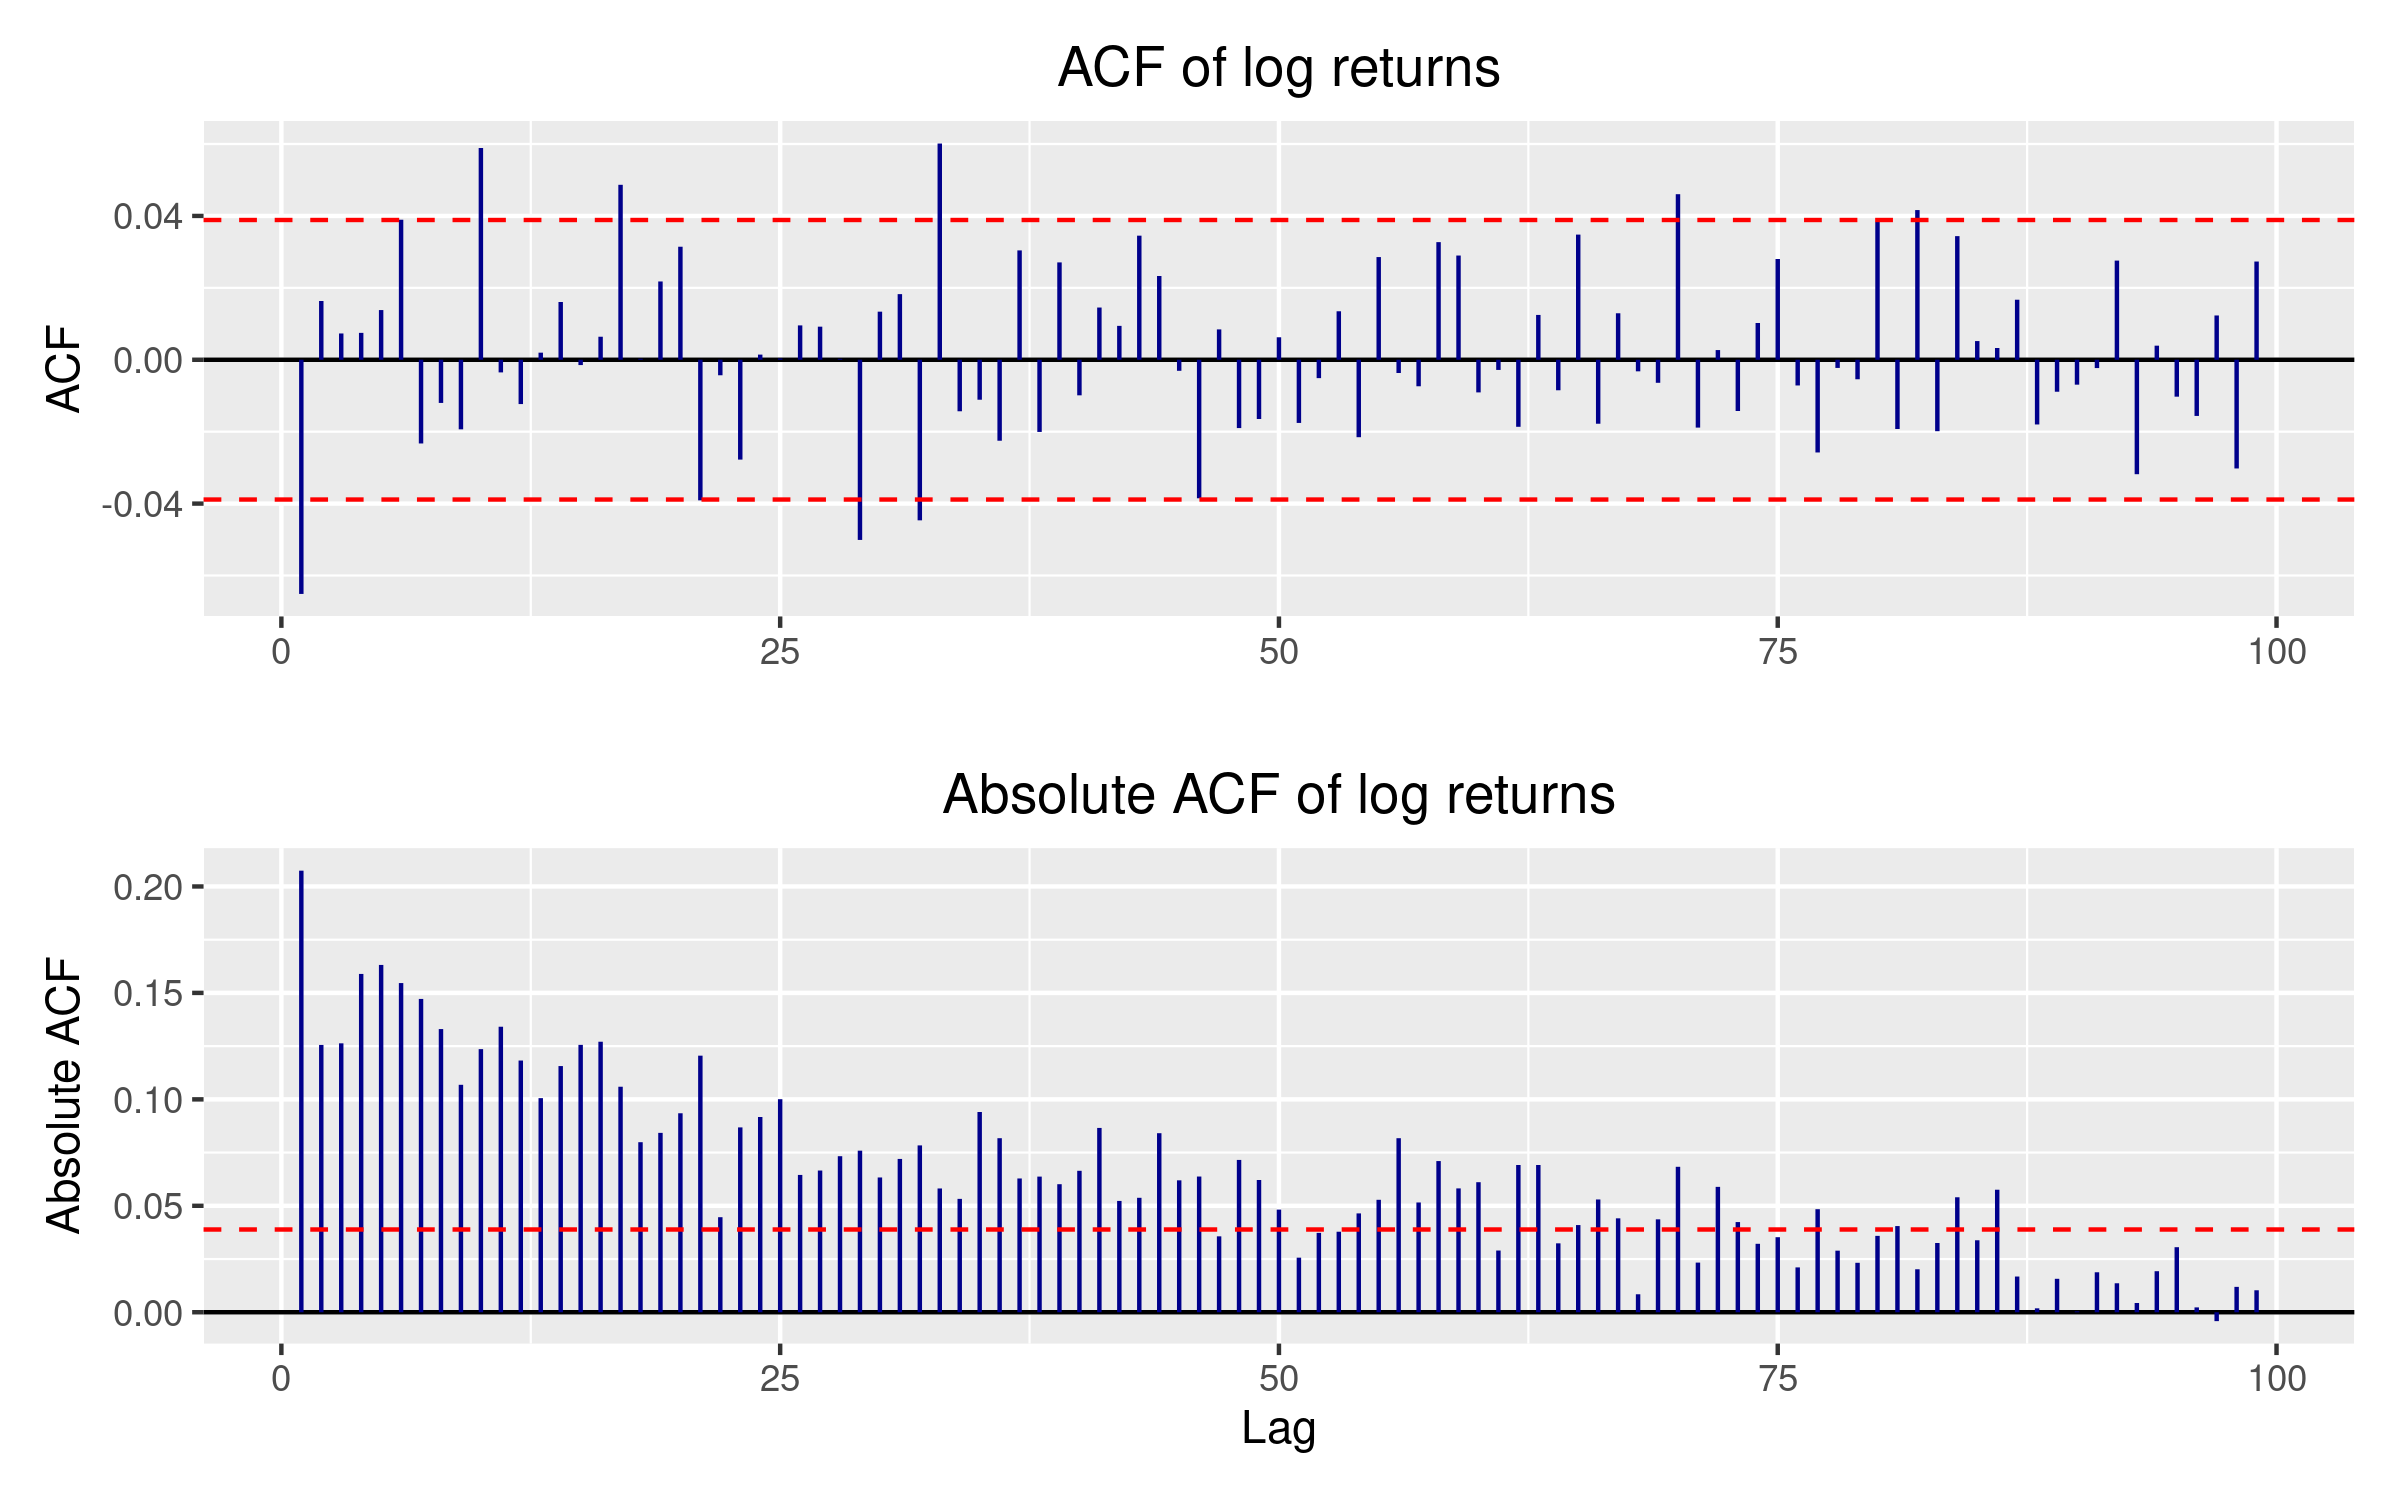
\includegraphics[scale=0.73]{{empirical_results/acf.png}}
	\subcaption*{Notes: The upper plot shows the autocorrelation function (ACF) of the raw percentage log-returns up to lag 100. The lower plot presents the ACF of the absolute percentage log-returns up to lag 100. The horizontal dashed blue lines represent the 95$\%$ (individual) significance bounds given by $\pm \frac{1.96}{\sqrt{T}}$. T is the total number of returns. Note that we do not account for multiple testing or conditional heteroscedasticity. In general, both would lead to larger significance bounds}
\end{figure}

\begin{figure}[!htb]
	\caption{Smoothed probabilities and annualized volatilities, Bayesian Estimation}
	\label{figure:smooth_probs_mcmc}
	\centering
	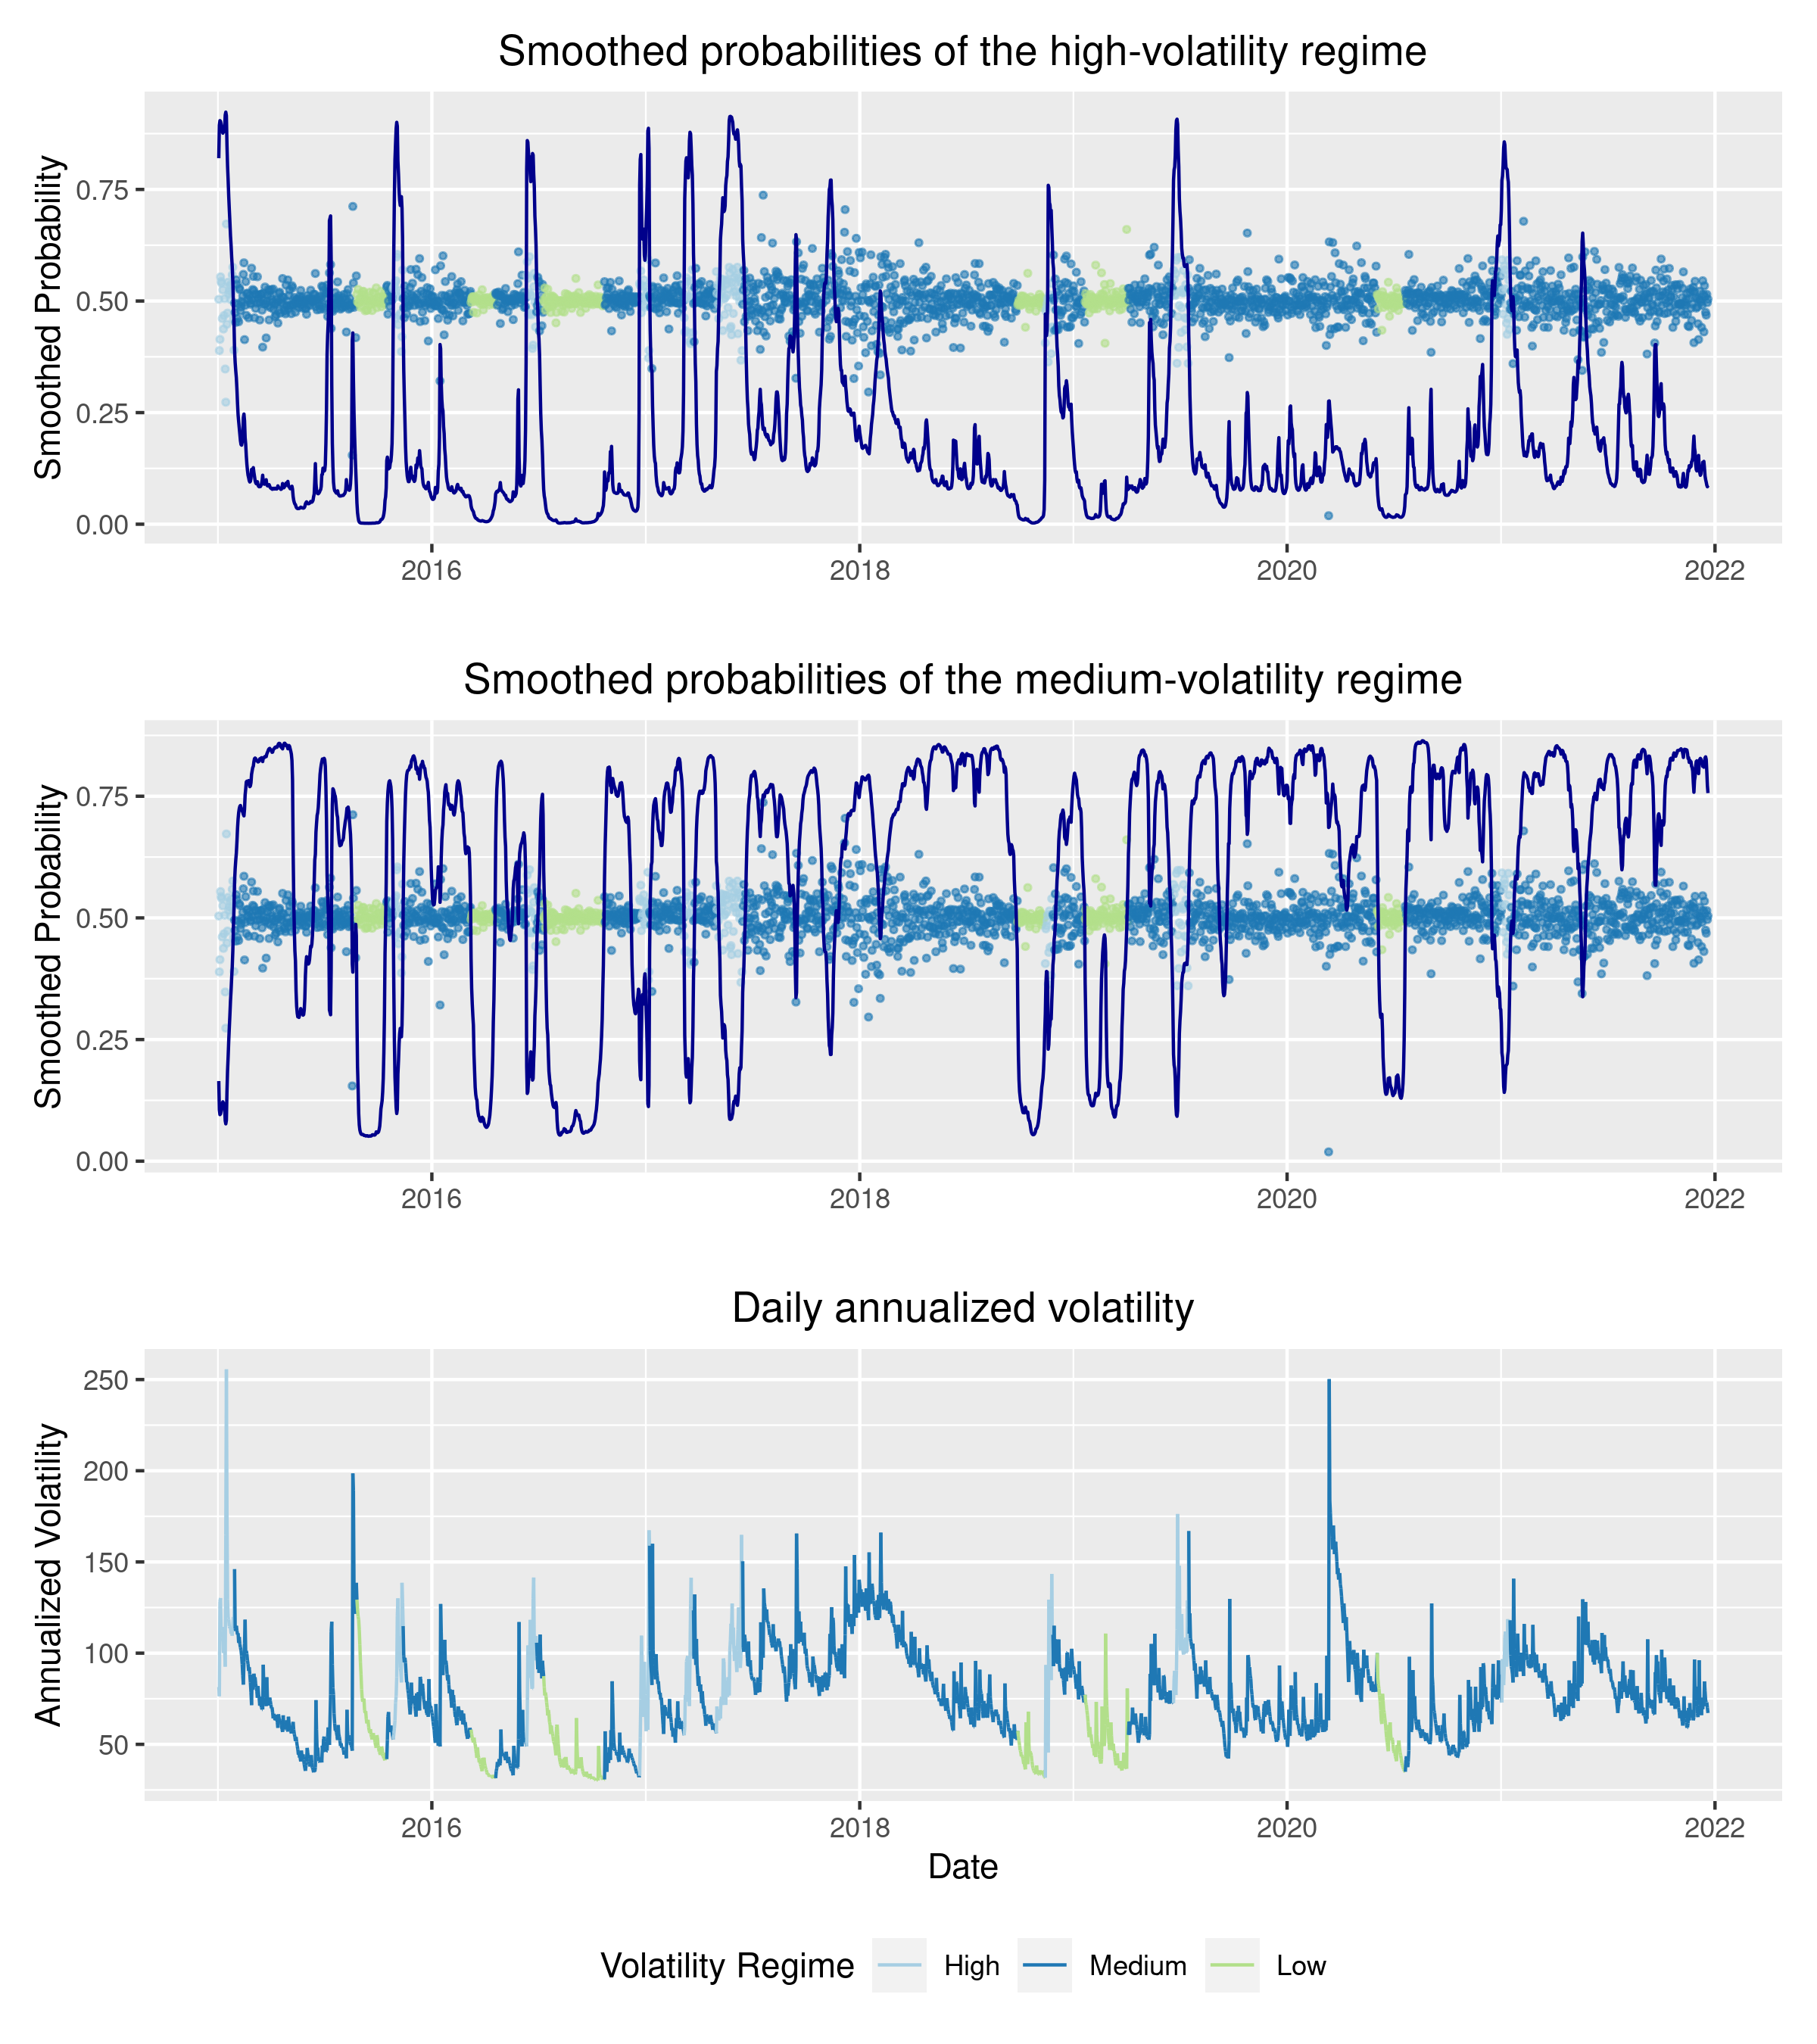
\includegraphics[scale=0.73]{{empirical_results/mcmc_prob_vol_plot.png}}
	\subcaption*{Notes: The time series range from January 01, 2015 to Dec 20, 2021. The graphs are computed from the three-regime SJRGARCH model with a standardized skewed Student's t-distribution. Parameters in the models are estimated using Bayesian Estimation. The estimated smoothed probabilities of the high- and medium-volatility regimes (3rd and 2nd regimes) are shown in the upper and middle graphs, respectively, together with the BTC-USD log-returns (points). The bottom graph shows the annualized volatilities in percentage. The colors of each point and color segments of the annualized volatility series indicate the regime to which the points or segments are predicted to belong.}
\end{figure}

\begin{figure}[!ht]
    \caption{Value-at-risk forecasts, Bayesian Estimation}
    \label{figure:mcmc_oos_var_ml}
    \centering
    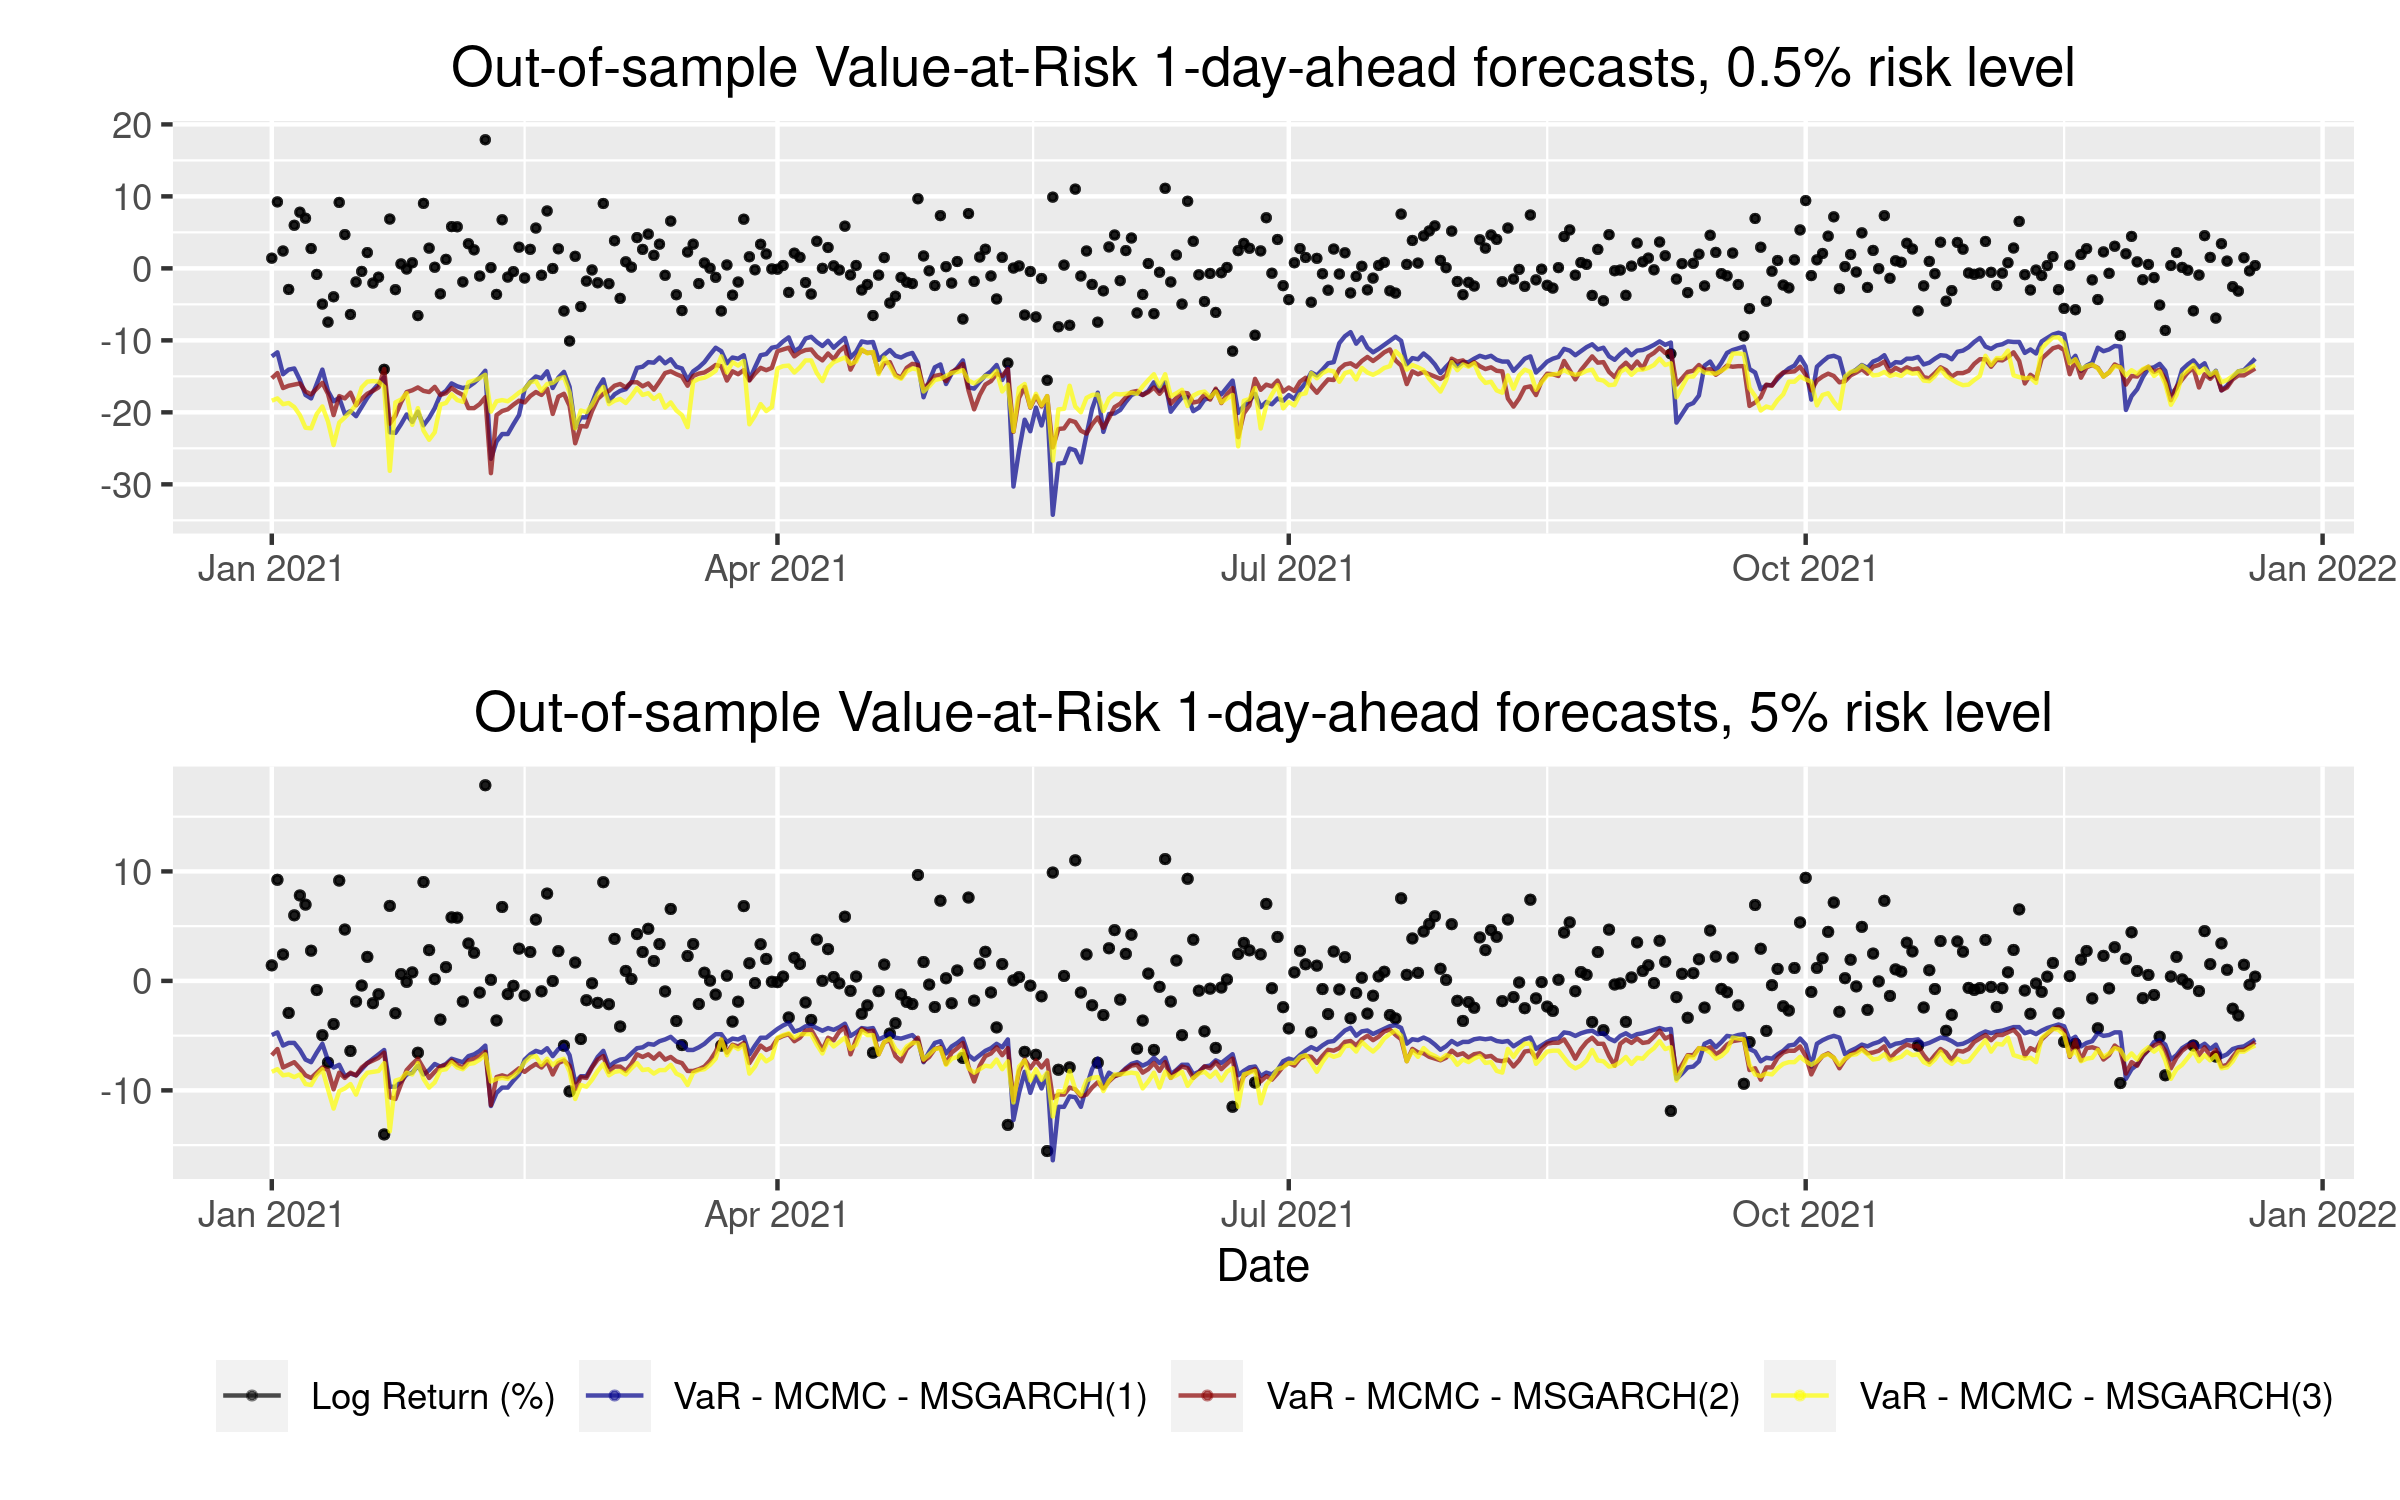
\includegraphics[scale=0.73]{{empirical_results/mcmc_oos_VaR.png}}
    \subcaption* {Notes: The time series range from January 01, 2015 to Dec 20, 2021. The out-of-sample period ranges from Jan 01, 2021 to Dec 20, 2021. The top graph shows the one-day-ahead Value-at-risk (VaR) forecasts at the 0.5$\%$ risk level computed with the single regime (blue line), two-regime (red line) and three-regime (green line) GJR-GARCH-sk$\mathcal{S}$ models. The percentage log-returns are depicted as the dots. GJR-GARCH is an extenstion of GARCH model of \cite{glosten1993relation} and sk$\mathcal{S}$ is the standardized skewed Student's t-distribution. The bottom graph depicts the one-day-ahead VaR forecasts at the 5$\%$ risk level.}
\end{figure}


\begin{table}[htbp]
\center
\begin{threeparttable}
\caption{Parameter estimates, Bayesian Estimation}
\label{table:params_mcmc}
\begin{tabular}{llllrrrrrr}
\hline
               & \multicolumn{3}{c}{Single-regime}                                                                     & \multicolumn{3}{c}{Two-regime}                                        & \multicolumn{3}{c}{Three-regime}                              \\
               & \multicolumn{1}{r}{\textit{Mean}} & \multicolumn{1}{r}{\textit{Q1}} & \multicolumn{1}{r}{\textit{Q3}} & \textit{Mean}         & \textit{Q1}           & \textit{Q3}           & \textit{Mean} & \textit{Q1}           & \textit{Q3}           \\ \hline
\multicolumn{10}{c}{\textit{Regime $k=1$}}                                                                                                                                                                                                                     \\
$\omega_1$     & \multicolumn{1}{r}{0.01}          & \multicolumn{1}{r}{0.01}        & \multicolumn{1}{r}{0.02}        & 5.92                  & 0.15                  & 12.18                 & 0.07          & 0.05                  & 0.08                  \\
$\alpha_1$     & \multicolumn{1}{r}{0.07}          & \multicolumn{1}{r}{0.06}        & \multicolumn{1}{r}{0.07}        & 0.08                  & 0.07                  & 0.10                  & 0.01          & 0.01                  & 0.01                  \\
$\gamma_1$     & \multicolumn{1}{r}{0.01}          & \multicolumn{1}{r}{0.01}        & \multicolumn{1}{r}{0.01}        & 0.10                  & 0.00                  & 0.19                  & 0.00          & 0.00                  & 0.00                  \\
$\beta_1$      & \multicolumn{1}{r}{0.93}          & \multicolumn{1}{r}{0.92}        & \multicolumn{1}{r}{0.93}        & 0.67                  & 0.40                  & 0.91                  & 0.96          & 0.95                  & 0.96                  \\
$\nu_1$        & \multicolumn{1}{r}{3.84}          & \multicolumn{1}{r}{3.72}        & \multicolumn{1}{r}{3.95}        & 4.03                  & 2.78                  & 5.08                  & 2.87          & 2.53                  & 3.04                  \\
$\delta_1$     & \multicolumn{1}{r}{0.95}          & \multicolumn{1}{r}{0.94}        & \multicolumn{1}{r}{0.97}        & 0.91                  & 0.89                  & 0.96                  & 0.99          & 0.95                  & 1.02                  \\
$p_11$         & -                                 & -                               & -                               & 0.95                  & 0.96                  & 0.98                  & 0.95          & 0.95                  & 0.96                  \\
$\text{aUV}_1$ & \multicolumn{1}{r}{43.38}         & -                               & -                               & 89.64                 & \multicolumn{1}{l}{-} & \multicolumn{1}{l}{-} & 26.98         & \multicolumn{1}{l}{-} & \multicolumn{1}{l}{-} \\
\multicolumn{10}{c}{\textit{Regime $k=2$}}                                                                                                                                                                                                                     \\
$\omega_1$     & -                                 & -                               & -                               & 6.01                  & 0.26                  & 11.06                 & 1.92          & 0.08                  & 0.13                  \\
$\alpha_1$     & -                                 & -                               & -                               & 0.09                  & 0.07                  & 0.11                  & 0.05          & 0.03                  & 0.04                  \\
$\gamma_1$     & -                                 & -                               & -                               & 0.12                  & 0.00                  & 0.22                  & 0.01          & 0.00                  & 0.00                  \\
$\beta_1$      & -                                 & -                               & -                               & 0.68                  & 0.47                  & 0.90                  & 0.89          & 0.95                  & 0.96                  \\
$\nu_1$        & -                                 & -                               & -                               & 4.17                  & 2.64                  & 5.28                  & 4.27          & 3.51                  & 4.19                  \\
$\delta_1$     & -                                 & -                               & -                               & 0.90                  & 0.87                  & 0.95                  & 0.93          & 0.91                  & 0.96                  \\
$p_22$         & -                                 & -                               & -                               & 0.92                  & 0.96                  & 0.98                  & 0.97          & 0.97                  & 0.98                  \\
$text{aUV}_2$  & -                                 & -                               & -                               & 113.80                & \multicolumn{1}{l}{-} & \multicolumn{1}{l}{-} & 71.18         & \multicolumn{1}{l}{-} & \multicolumn{1}{l}{-} \\
\multicolumn{10}{c}{\textit{Regime $k=3$}}                                                                                                                                                                                                                     \\
$\omega_1$     & -                                 & -                               & -                               & \multicolumn{1}{l}{-} & \multicolumn{1}{l}{-} & \multicolumn{1}{l}{-} & 27.16         & 23.44                 & 32.73                 \\
$\alpha_1$     & -                                 & -                               & -                               & \multicolumn{1}{l}{-} & \multicolumn{1}{l}{-} & \multicolumn{1}{l}{-} & 0.17          & 0.10                  & 0.22                  \\
$\gamma_1$     & -                                 & -                               & -                               & \multicolumn{1}{l}{-} & \multicolumn{1}{l}{-} & \multicolumn{1}{l}{-} & 0.16          & 0.11                  & 0.20                  \\
$\beta_1$      & -                                 & -                               & -                               & \multicolumn{1}{l}{-} & \multicolumn{1}{l}{-} & \multicolumn{1}{l}{-} & 0.11          & 0.02                  & 0.08                  \\
$\nu_1$        & -                                 & -                               & -                               & \multicolumn{1}{l}{-} & \multicolumn{1}{l}{-} & \multicolumn{1}{l}{-} & 8.39          & 5.74                  & 10.66                 \\
$\delta_1$     & -                                 & -                               & -                               & \multicolumn{1}{l}{-} & \multicolumn{1}{l}{-} & \multicolumn{1}{l}{-} & 0.75          & 0.68                  & 0.81                  \\
$p_33$         & -                                 & -                               & -                               & \multicolumn{1}{l}{-} & \multicolumn{1}{l}{-} & \multicolumn{1}{l}{-} & 0.91          & 0.90                  & 0.93                  \\
$\text{aUV}_3$ & -                                 & -                               & -                               & \multicolumn{1}{l}{-} & \multicolumn{1}{l}{-} & \multicolumn{1}{l}{-} & 123.70        & \multicolumn{1}{l}{-} & \multicolumn{1}{l}{-} \\ \hline
\end{tabular}
\begin{tablenotes}
\small
\item Notes: The table presents the Bayesian Estimation parameter estimates of the $K$-regime GJR-GARCH-sk$\mathcal{S}$ models, $K = 1, 2, 3$. GJR-GARCH is an extension of GARCH model proposed in \cite{glosten1993relation}. sk$\mathcal{S}$ is the standardized skewed Student's t-distribution with tail parameter $\nu$ and asymmetry parameter $\delta$. $p_{kk}$ is the staying probability of state $k$. $aUV$ is the annualized unconditional volatility (in $\%$). Here, 1st and 3rd Quartiles are showed as uncertainty estimates instead of traditional standard deviation and t-statistics.
\end{tablenotes}
\end{threeparttable}
\end{table}


\begin{table}[p]
\centering
\begin{threeparttable}
\caption {Backtesting results for 1-step-ahead volatility forecasts, Bayesian Estimation}
\label{table:backtest_mcmc}
\begin{tabular}{llrrrr}
\hline
                & \multicolumn{1}{c}{VaR risk level} & \multicolumn{1}{c}{0.005} & \multicolumn{1}{c}{0.01} & \multicolumn{1}{c}{0.05} & \multicolumn{1}{c}{0.1} \\ \hline
MCMC-MSGARCH(1) & $LR_{UC}$                          & 0.5272                    & 0.2319                   & 0.2157                   & \textbf{0.0142}         \\
                & $LR_{CC}$                          & 0.8165                    & 0.4412                   & 0.4180                   & \textbf{0.0495}         \\
MCMC-MSGARCH(2) & $LR_{UC}$                          & 0.8652                    & 0.8098                   & 0.8636                   & \textbf{0.0491}         \\
                & $LR_{CC}$                          & 0.9745                    & 0.9279                   & 0.4168                   & 0.1209                  \\
MCMC-MSGARCH(3) & $LR_{UC}$                          & \textbf{0.0596}           & 0.7671                   & 0.4994                   & 0.6486                  \\
                & $LR_{CC}$                          & 0.1696                    & 0.9328                   & 0.4090                   & 0.7991                  \\ \hline
\end{tabular}
\begin{tablenotes}
\small
\item Notes: The table presents the backtesting results for the 1-step-ahead value-at-risk ( VaR ) at risk levels 0.5$\%$, 1$\%$, 5$\%$ and 10$\%$. Shown are the $p$-values of the Likelihood Ratio test of Unconditional Coverage $(LR_{UC})$ and the Likelihood Ratio test of Conditional Coverage $(LR_{CC})$ for the $K$-regime GJR-GARCH \citep{glosten1993relation} models, $K = 1,2,3$, with a standardized skewed Student's t-distribution.
\end{tablenotes}
\end{threeparttable}
\end{table}


\begin{table}[b]
\centering
\caption{Expected and observed number of violations, Bayesian Estimation}
\label{table:hitrate_mcmc}
\begin{tabular}{@{}rlclclclcl@{}}
\toprule
\multicolumn{2}{r}{VaR risk level}     & \multicolumn{2}{c}{0.005} & \multicolumn{2}{c}{0.01}  & \multicolumn{2}{c}{0.05} & \multicolumn{2}{c}{0.1}   \\ \midrule
\multicolumn{2}{r}{\textit{Expected number of hits}} & \multicolumn{2}{c}{5.31}  & \multicolumn{2}{c}{10.62} & \multicolumn{2}{c}{53.1} & \multicolumn{2}{c}{106.2} \\
\multicolumn{2}{r}{\textit{Observed number of hits}} & \multicolumn{8}{c}{}                                                                                         \\
\multicolumn{2}{r}{MCMC-MSGARCH(1)}         & \multicolumn{2}{c}{1}     & \multicolumn{2}{c}{6}     & \multicolumn{2}{c}{23}   & \multicolumn{2}{c}{50}    \\
\multicolumn{2}{r}{MCMC-MSGARCH(2)}         & \multicolumn{2}{c}{2}     & \multicolumn{2}{c}{4}     & \multicolumn{2}{c}{17}   & \multicolumn{2}{c}{47}    \\
\multicolumn{2}{r}{MCMC-MSGARCH(3)}         & \multicolumn{2}{c}{0}     & \multicolumn{2}{c}{3}     & \multicolumn{2}{c}{15}   & \multicolumn{2}{c}{38}    \\ \bottomrule
\end{tabular}
\end{table}

\end{document}